\documentclass[11pt,a4paper]{article}
\usepackage[T1]{fontenc}
\usepackage[utf8]{inputenc}
\usepackage{lmodern}
\usepackage{microtype}
\usepackage[a4paper,margin=2.3cm]{geometry}
\usepackage{graphicx}
\usepackage{booktabs}
\usepackage{tabularx}
\usepackage{array}
\usepackage{multirow}
\usepackage{float}
\usepackage{caption}
\usepackage{subcaption}
\usepackage{enumitem}
\usepackage{amsmath,amssymb}
\usepackage{xcolor}
\usepackage{tikz}
\usetikzlibrary{positioning,arrows.meta,fit,backgrounds,calc}
\usepackage{fancyhdr}
\usepackage{titlesec}
\usepackage{listings}
\usepackage[hidelinks]{hyperref}

\definecolor{diublue}{HTML}{0B4EA2}
\definecolor{diugreen}{HTML}{2E9E44}
\definecolor{ink}{HTML}{0B0B0B}
\definecolor{ink2}{HTML}{52514E}
\definecolor{boxblue}{HTML}{E8F1FC}
\definecolor{boxorange}{HTML}{FDEEE6}
\definecolor{boxgreen}{HTML}{E6F6EF}
\definecolor{rulegray}{HTML}{D9D8D4}

\titleformat{\section}{\Large\bfseries\color{diublue}}{\thesection}{0.8em}{}
\titleformat{\subsection}{\large\bfseries\color{ink}}{\thesubsection}{0.7em}{}
\titleformat{\subsubsection}{\normalsize\bfseries\color{ink}}{\thesubsubsection}{0.6em}{}
\setlength{\parskip}{0.45em}
\setlength{\parindent}{0pt}
\captionsetup{font=small,labelfont=bf,margin=0.5cm}
\setlist{itemsep=0.15em,topsep=0.3em}

\lstset{basicstyle=\ttfamily\small,columns=fullflexible,breaklines=true,frame=single,
  rulecolor=\color{rulegray},backgroundcolor=\color{boxblue!40},xleftmargin=0.5em,xrightmargin=0.5em}

\pagestyle{fancy}
\fancyhf{}
\fancyhead[L]{\small\color{ink2}Deep Learning --- Group Assignment 1 (CT-1)}
\fancyhead[R]{\small\color{ink2}Task 2: Transfer Learning}
\fancyfoot[L]{\small\color{ink2}Shakib Howlader (262-25-013)}
\fancyfoot[R]{\small\color{ink2}\thepage}
\renewcommand{\headrulewidth}{0.4pt}

\makeatletter
\newcommand{\inputrows}[1]{\@@input #1 }  % primitive \input: safe inside tabular rows
\makeatother
\setlength{\emergencystretch}{2em}

\newcommand{\repo}{https://github.com/mr-shakib/dermamnist-transfer-learning}
\newcommand{\MajorityAcc}{66.9}
\newcommand{\NumRuns}{7}
\newcommand{\DatasetSizeMB}{1{,}091}
\newcommand{\TorchVersion}{2.14.1}
\newcommand{\BestLabel}{ResNet-50 (fine-tune)}
\newcommand{\BestTTA}{with 8-view TTA}
\newcommand{\ScratchAcc}{73.6}
\newcommand{\ScratchBalAcc}{49.4}
\newcommand{\ScratchFOne}{48.0}
\newcommand{\ScratchAUC}{0.908}
\newcommand{\ScratchECE}{0.163}
\newcommand{\ScratchWFOne}{73.6}
\newcommand{\ScratchKappa}{0.502}
\newcommand{\ScratchAccTTA}{74.8}
\newcommand{\ScratchBalAccTTA}{52.2}
\newcommand{\ScratchFOneTTA}{50.6}
\newcommand{\ScratchAUCTTA}{0.911}
\newcommand{\ScratchECETTA}{0.176}
\newcommand{\ScratchWFOneTTA}{74.7}
\newcommand{\ScratchKappaTTA}{0.525}
\newcommand{\ScratchAccVal}{74.3}
\newcommand{\ScratchBalAccVal}{47.2}
\newcommand{\ScratchFOneVal}{48.6}
\newcommand{\ScratchAUCVal}{0.914}
\newcommand{\ScratchECEVal}{0.174}
\newcommand{\ScratchWFOneVal}{74.2}
\newcommand{\ScratchKappaVal}{0.509}
\newcommand{\ScratchFOneCI}{[44.6, 51.0]}
\newcommand{\ScratchAccCI}{[71.5, 75.5]}
\newcommand{\ScratchAUCCI}{[0.894, 0.921]}
\newcommand{\ScratchFOneTTACI}{[47.4, 53.2]}
\newcommand{\ScratchAccTTACI}{[72.8, 76.8]}
\newcommand{\ScratchBalAccTTACI}{[49.1, 55.1]}
\newcommand{\ScratchAUCTTACI}{[0.897, 0.924]}
\newcommand{\ScratchBestEpoch}{19}
\newcommand{\ScratchEpochTime}{19}
\newcommand{\ScratchTrainMin}{8.9}
\newcommand{\ScratchFOneAkiec}{37.9}
\newcommand{\ScratchFOneBcc}{40.6}
\newcommand{\ScratchFOneBkl}{50.0}
\newcommand{\ScratchFOneDf}{0.0}
\newcommand{\ScratchFOneMel}{48.4}
\newcommand{\ScratchFOneNv}{87.2}
\newcommand{\ScratchFOneVasc}{72.1}
\newcommand{\RFrozenAcc}{76.5}
\newcommand{\RFrozenBalAcc}{56.6}
\newcommand{\RFrozenFOne}{55.9}
\newcommand{\RFrozenAUC}{0.920}
\newcommand{\RFrozenECE}{0.198}
\newcommand{\RFrozenWFOne}{76.8}
\newcommand{\RFrozenKappa}{0.563}
\newcommand{\RFrozenAccTTA}{77.2}
\newcommand{\RFrozenBalAccTTA}{57.4}
\newcommand{\RFrozenFOneTTA}{57.8}
\newcommand{\RFrozenAUCTTA}{0.926}
\newcommand{\RFrozenECETTA}{0.207}
\newcommand{\RFrozenWFOneTTA}{77.4}
\newcommand{\RFrozenKappaTTA}{0.575}
\newcommand{\RFrozenAccVal}{76.4}
\newcommand{\RFrozenBalAccVal}{55.4}
\newcommand{\RFrozenFOneVal}{55.4}
\newcommand{\RFrozenAUCVal}{0.918}
\newcommand{\RFrozenECEVal}{0.201}
\newcommand{\RFrozenWFOneVal}{76.7}
\newcommand{\RFrozenKappaVal}{0.561}
\newcommand{\RFrozenFOneCI}{[51.3, 60.3]}
\newcommand{\RFrozenAccCI}{[74.3, 78.3]}
\newcommand{\RFrozenAUCCI}{[0.905, 0.934]}
\newcommand{\RFrozenFOneTTACI}{[53.1, 62.2]}
\newcommand{\RFrozenAccTTACI}{[75.3, 79.0]}
\newcommand{\RFrozenBalAccTTACI}{[53.3, 62.2]}
\newcommand{\RFrozenAUCTTACI}{[0.912, 0.939]}
\newcommand{\RFrozenBestEpoch}{9}
\newcommand{\RFrozenEpochTime}{20}
\newcommand{\RFrozenTrainMin}{3.9}
\newcommand{\RFrozenFOneAkiec}{46.2}
\newcommand{\RFrozenFOneBcc}{52.5}
\newcommand{\RFrozenFOneBkl}{57.7}
\newcommand{\RFrozenFOneDf}{38.9}
\newcommand{\RFrozenFOneMel}{47.8}
\newcommand{\RFrozenFOneNv}{89.2}
\newcommand{\RFrozenFOneVasc}{59.2}
\newcommand{\EFrozenAcc}{75.3}
\newcommand{\EFrozenBalAcc}{63.5}
\newcommand{\EFrozenFOne}{59.4}
\newcommand{\EFrozenAUC}{0.929}
\newcommand{\EFrozenECE}{0.171}
\newcommand{\EFrozenWFOne}{76.5}
\newcommand{\EFrozenKappa}{0.561}
\newcommand{\EFrozenAccTTA}{76.7}
\newcommand{\EFrozenBalAccTTA}{62.6}
\newcommand{\EFrozenFOneTTA}{59.3}
\newcommand{\EFrozenAUCTTA}{0.935}
\newcommand{\EFrozenECETTA}{0.188}
\newcommand{\EFrozenWFOneTTA}{77.7}
\newcommand{\EFrozenKappaTTA}{0.581}
\newcommand{\EFrozenAccVal}{76.0}
\newcommand{\EFrozenBalAccVal}{62.9}
\newcommand{\EFrozenFOneVal}{59.1}
\newcommand{\EFrozenAUCVal}{0.932}
\newcommand{\EFrozenECEVal}{0.183}
\newcommand{\EFrozenWFOneVal}{77.0}
\newcommand{\EFrozenKappaVal}{0.571}
\newcommand{\EFrozenFOneCI}{[55.2, 63.0]}
\newcommand{\EFrozenAccCI}{[73.4, 77.2]}
\newcommand{\EFrozenAUCCI}{[0.916, 0.941]}
\newcommand{\EFrozenFOneTTACI}{[55.2, 63.0]}
\newcommand{\EFrozenAccTTACI}{[74.9, 78.6]}
\newcommand{\EFrozenBalAccTTACI}{[58.6, 66.8]}
\newcommand{\EFrozenAUCTTACI}{[0.922, 0.947]}
\newcommand{\EFrozenBestEpoch}{10}
\newcommand{\EFrozenEpochTime}{10}
\newcommand{\EFrozenTrainMin}{1.9}
\newcommand{\EFrozenFOneAkiec}{48.6}
\newcommand{\EFrozenFOneBcc}{57.3}
\newcommand{\EFrozenFOneBkl}{56.5}
\newcommand{\EFrozenFOneDf}{53.8}
\newcommand{\EFrozenFOneMel}{46.2}
\newcommand{\EFrozenFOneNv}{88.4}
\newcommand{\EFrozenFOneVasc}{64.8}
\newcommand{\RFineAcc}{86.1}
\newcommand{\RFineBalAcc}{76.3}
\newcommand{\RFineFOne}{77.2}
\newcommand{\RFineAUC}{0.955}
\newcommand{\RFineECE}{0.084}
\newcommand{\RFineWFOne}{86.4}
\newcommand{\RFineKappa}{0.745}
\newcommand{\RFineAccTTA}{87.0}
\newcommand{\RFineBalAccTTA}{79.2}
\newcommand{\RFineFOneTTA}{80.1}
\newcommand{\RFineAUCTTA}{0.962}
\newcommand{\RFineECETTA}{0.102}
\newcommand{\RFineWFOneTTA}{87.3}
\newcommand{\RFineKappaTTA}{0.761}
\newcommand{\RFineAccVal}{85.2}
\newcommand{\RFineBalAccVal}{78.8}
\newcommand{\RFineFOneVal}{79.5}
\newcommand{\RFineAUCVal}{0.961}
\newcommand{\RFineECEVal}{0.087}
\newcommand{\RFineWFOneVal}{86.0}
\newcommand{\RFineKappaVal}{0.733}
\newcommand{\RFineFOneCI}{[73.4, 80.5]}
\newcommand{\RFineAccCI}{[84.6, 87.5]}
\newcommand{\RFineAUCCI}{[0.939, 0.968]}
\newcommand{\RFineFOneTTACI}{[76.6, 83.0]}
\newcommand{\RFineAccTTACI}{[85.5, 88.4]}
\newcommand{\RFineBalAccTTACI}{[75.3, 82.9]}
\newcommand{\RFineAUCTTACI}{[0.948, 0.974]}
\newcommand{\RFineBestEpoch}{11}
\newcommand{\RFineEpochTime}{66}
\newcommand{\RFineTrainMin}{13.8}
\newcommand{\RFineFOneAkiec}{58.9}
\newcommand{\RFineFOneBcc}{81.9}
\newcommand{\RFineFOneBkl}{73.6}
\newcommand{\RFineFOneDf}{74.4}
\newcommand{\RFineFOneMel}{69.0}
\newcommand{\RFineFOneNv}{93.3}
\newcommand{\RFineFOneVasc}{89.3}
\newcommand{\EFineAcc}{84.8}
\newcommand{\EFineBalAcc}{76.0}
\newcommand{\EFineFOne}{72.9}
\newcommand{\EFineAUC}{0.959}
\newcommand{\EFineECE}{0.103}
\newcommand{\EFineWFOne}{85.0}
\newcommand{\EFineKappa}{0.718}
\newcommand{\EFineAccTTA}{86.1}
\newcommand{\EFineBalAccTTA}{79.2}
\newcommand{\EFineFOneTTA}{75.6}
\newcommand{\EFineAUCTTA}{0.966}
\newcommand{\EFineECETTA}{0.127}
\newcommand{\EFineWFOneTTA}{86.3}
\newcommand{\EFineKappaTTA}{0.744}
\newcommand{\EFineAccVal}{85.7}
\newcommand{\EFineBalAccVal}{78.6}
\newcommand{\EFineFOneVal}{73.4}
\newcommand{\EFineAUCVal}{0.971}
\newcommand{\EFineECEVal}{0.116}
\newcommand{\EFineWFOneVal}{85.8}
\newcommand{\EFineKappaVal}{0.739}
\newcommand{\EFineFOneCI}{[69.0, 76.3]}
\newcommand{\EFineAccCI}{[83.1, 86.3]}
\newcommand{\EFineAUCCI}{[0.948, 0.968]}
\newcommand{\EFineFOneTTACI}{[71.7, 79.0]}
\newcommand{\EFineAccTTACI}{[84.6, 87.6]}
\newcommand{\EFineBalAccTTACI}{[76.0, 82.3]}
\newcommand{\EFineAUCTTACI}{[0.957, 0.975]}
\newcommand{\EFineBestEpoch}{11}
\newcommand{\EFineEpochTime}{32}
\newcommand{\EFineTrainMin}{6.6}
\newcommand{\EFineFOneAkiec}{54.7}
\newcommand{\EFineFOneBcc}{78.1}
\newcommand{\EFineFOneBkl}{72.0}
\newcommand{\EFineFOneDf}{59.0}
\newcommand{\EFineFOneMel}{64.5}
\newcommand{\EFineFOneNv}{92.9}
\newcommand{\EFineFOneVasc}{88.9}
\newcommand{\RGradAcc}{83.0}
\newcommand{\RGradBalAcc}{74.1}
\newcommand{\RGradFOne}{73.2}
\newcommand{\RGradAUC}{0.958}
\newcommand{\RGradECE}{0.133}
\newcommand{\RGradWFOne}{83.7}
\newcommand{\RGradKappa}{0.694}
\newcommand{\RGradAccTTA}{84.2}
\newcommand{\RGradBalAccTTA}{76.6}
\newcommand{\RGradFOneTTA}{76.5}
\newcommand{\RGradAUCTTA}{0.968}
\newcommand{\RGradECETTA}{0.152}
\newcommand{\RGradWFOneTTA}{84.9}
\newcommand{\RGradKappaTTA}{0.715}
\newcommand{\RGradAccVal}{82.4}
\newcommand{\RGradBalAccVal}{71.5}
\newcommand{\RGradFOneVal}{70.6}
\newcommand{\RGradAUCVal}{0.951}
\newcommand{\RGradECEVal}{0.127}
\newcommand{\RGradWFOneVal}{83.0}
\newcommand{\RGradKappaVal}{0.684}
\newcommand{\RGradFOneCI}{[69.3, 76.4]}
\newcommand{\RGradAccCI}{[81.3, 84.6]}
\newcommand{\RGradAUCCI}{[0.946, 0.968]}
\newcommand{\RGradFOneTTACI}{[72.7, 79.5]}
\newcommand{\RGradAccTTACI}{[82.7, 85.8]}
\newcommand{\RGradBalAccTTACI}{[72.6, 80.3]}
\newcommand{\RGradAUCTTACI}{[0.958, 0.977]}
\newcommand{\RGradBestEpoch}{6}
\newcommand{\RGradEpochTime}{45}
\newcommand{\RGradTrainMin}{9.7}
\newcommand{\RGradFOneAkiec}{64.8}
\newcommand{\RGradFOneBcc}{72.2}
\newcommand{\RGradFOneBkl}{70.4}
\newcommand{\RGradFOneDf}{65.1}
\newcommand{\RGradFOneMel}{62.4}
\newcommand{\RGradFOneNv}{91.5}
\newcommand{\RGradFOneVasc}{86.2}
\newcommand{\RNoWAcc}{86.9}
\newcommand{\RNoWBalAcc}{71.8}
\newcommand{\RNoWFOne}{75.7}
\newcommand{\RNoWAUC}{0.971}
\newcommand{\RNoWECE}{0.024}
\newcommand{\RNoWWFOne}{87.0}
\newcommand{\RNoWKappa}{0.754}
\newcommand{\RNoWAccTTA}{88.8}
\newcommand{\RNoWBalAccTTA}{74.8}
\newcommand{\RNoWFOneTTA}{78.5}
\newcommand{\RNoWAUCTTA}{0.979}
\newcommand{\RNoWECETTA}{0.037}
\newcommand{\RNoWWFOneTTA}{88.8}
\newcommand{\RNoWKappaTTA}{0.788}
\newcommand{\RNoWAccVal}{86.6}
\newcommand{\RNoWBalAccVal}{75.2}
\newcommand{\RNoWFOneVal}{77.1}
\newcommand{\RNoWAUCVal}{0.970}
\newcommand{\RNoWECEVal}{0.035}
\newcommand{\RNoWWFOneVal}{86.7}
\newcommand{\RNoWKappaVal}{0.750}
\newcommand{\RNoWFOneCI}{[71.7, 79.4]}
\newcommand{\RNoWAccCI}{[85.5, 88.4]}
\newcommand{\RNoWAUCCI}{[0.963, 0.979]}
\newcommand{\RNoWFOneTTACI}{[74.8, 82.0]}
\newcommand{\RNoWAccTTACI}{[87.4, 90.0]}
\newcommand{\RNoWBalAccTTACI}{[71.1, 79.4]}
\newcommand{\RNoWAUCTTACI}{[0.973, 0.985]}
\newcommand{\RNoWBestEpoch}{11}
\newcommand{\RNoWEpochTime}{67}
\newcommand{\RNoWTrainMin}{14.1}
\newcommand{\RNoWFOneAkiec}{58.1}
\newcommand{\RNoWFOneBcc}{81.0}
\newcommand{\RNoWFOneBkl}{75.4}
\newcommand{\RNoWFOneDf}{68.4}
\newcommand{\RNoWFOneMel}{68.7}
\newcommand{\RNoWFOneNv}{94.3}
\newcommand{\RNoWFOneVasc}{84.0}
\newcommand{\BestPrecAkiec}{93.8}
\newcommand{\BestRecAkiec}{45.5}
\newcommand{\BestFOneAkiec}{61.2}
\newcommand{\BestAUCAkiec}{0.863}
\newcommand{\BestPrecBcc}{79.8}
\newcommand{\BestRecBcc}{88.3}
\newcommand{\BestFOneBcc}{83.9}
\newcommand{\BestAUCBcc}{0.989}
\newcommand{\BestPrecBkl}{72.8}
\newcommand{\BestRecBkl}{84.1}
\newcommand{\BestFOneBkl}{78.1}
\newcommand{\BestAUCBkl}{0.979}
\newcommand{\BestPrecDf}{86.4}
\newcommand{\BestRecDf}{82.6}
\newcommand{\BestFOneDf}{84.4}
\newcommand{\BestAUCDf}{0.971}
\newcommand{\BestPrecMel}{61.0}
\newcommand{\BestRecMel}{80.7}
\newcommand{\BestFOneMel}{69.5}
\newcommand{\BestAUCMel}{0.959}
\newcommand{\BestPrecNv}{96.1}
\newcommand{\BestRecNv}{90.6}
\newcommand{\BestFOneNv}{93.3}
\newcommand{\BestAUCNv}{0.977}
\newcommand{\BestPrecVasc}{100.0}
\newcommand{\BestRecVasc}{82.8}
\newcommand{\BestFOneVasc}{90.6}
\newcommand{\BestAUCVasc}{1.000}
\newcommand{\SilImageNet}{-0.039}
\newcommand{\SilFineTuned}{0.080}
\newcommand{\TotalTrainMin}{59}


\begin{document}

%======================== COVER PAGE ========================
\begin{titlepage}
\centering

\includegraphics[width=0.30\textwidth]{figures/diu_cse_logo.png}\par
\vspace{0.6cm}
{\LARGE\bfseries\color{diublue} Daffodil International University\par}
\vspace{0.15cm}
{\large Department of Computer Science and Engineering\par}
{\normalsize Faculty of Science and Information Technology\par}
\vspace{0.9cm}
{\large\bfseries M.Sc.\ in Computer Science and Engineering\par}
{\large Course: Deep Learning \quad$\cdot$\quad Fall 2026\par}
\vspace{0.5cm}
{\color{diugreen}\rule{0.8\textwidth}{1.2pt}\par}
\vspace{0.35cm}
{\large\bfseries Group Assignment 1 (CT-1)\par}
{\normalsize Task 2 --- CNN / Transfer Learning / Fine-tuning\par}
\vspace{0.45cm}
{\Large\bfseries\color{ink} Transfer Learning for Dermatoscopic\\[0.15cm] Skin-Lesion Classification\par}
\vspace{0.2cm}
{\large Fine-tuning ImageNet-pretrained CNNs on DermaMNIST (HAM10000)\par}
\vspace{0.35cm}
{\color{diugreen}\rule{0.8\textwidth}{1.2pt}\par}
\vspace{0.9cm}

{\large\bfseries Submitted by\par}
\vspace{0.25cm}
\begin{tabular}{>{\raggedright\arraybackslash}p{5.2cm} >{\raggedright\arraybackslash}p{4.0cm}}
\toprule
\textbf{Member name} & \textbf{Student ID} \\
\midrule
Shakib Howlader & 262-25-013 \\
\bottomrule
\end{tabular}
\par\vspace{0.8cm}

{\large\bfseries Submitted to\par}
\vspace{0.15cm}
Course Instructor, Deep Learning\\
Department of Computer Science and Engineering\\
Daffodil International University\par
\vfill
\begin{tabular}{rl}
\textbf{Date of submission:} & 26 October 2026 \\
\textbf{Codebase:} & \href{\repo}{\texttt{github.com/mr-shakib/dermamnist-transfer-learning}} \\
\end{tabular}
\end{titlepage}

%======================== ABSTRACT + TOC ========================
\pagenumbering{roman}
\section*{Abstract}
\addcontentsline{toc}{section}{Abstract}
Skin-lesion datasets are small and dominated by benign nevi, which makes it hard to train deep networks from
scratch. This report addresses \textbf{Task~2 (CNN / Transfer Learning / Fine-tuning)} by fine-tuning
ImageNet-pretrained CNNs on \textbf{DermaMNIST}, the seven-class MedMNIST version of the HAM10000 dermatoscopic
dataset (10{,}015 images, 224$\times$224). A data analysis shows a 58.7\,:\,1 class imbalance, a strong colour
shift from ImageNet, and a small amount of same-lesion leakage between the official splits. Under one
reproducible pipeline (class-weighted loss, augmentation, validation-based model selection), we compare seven
configurations: a CNN trained from scratch; feature extraction, full fine-tuning with discriminative learning
rates and gradual unfreezing of ResNet-50 and EfficientNet-B0; and a class-weighting ablation. Transfer learning
is decisive. Test macro-F1 rises from \ScratchFOne\% (scratch) to \RFrozenFOne\% with a frozen ResNet-50 and to
\RFineFOne\% with full fine-tuning. Gradual unfreezing (\RGradFOne\%) did not help within a 12-epoch budget, and
class weighting traded calibration for minority-class recall. The selected model, ResNet-50 fully fine-tuned with
8-view test-time augmentation, reaches \textbf{\RFineAccTTA\% accuracy}, \textbf{\RFineFOneTTA\% macro-F1}
(95\% CI \RFineFOneTTACI) and \textbf{macro-AUC \RFineAUCTTA} on the held-out test set, about 10 accuracy points
above the official MedMNIST v2 baselines. Grad-CAM and t-SNE show lesion-focused evidence and well-separated
class clusters after fine-tuning, while also pointing to hair and vignetting artefacts. All code, logs and
figures are public.

\vspace{0.3em}
\textbf{Keywords:} transfer learning, fine-tuning, convolutional neural networks, ResNet-50, EfficientNet,
dermatoscopy, skin-lesion classification, class imbalance, DermaMNIST, HAM10000.


\vspace{0.6cm}
\tableofcontents
\clearpage
\listoffigures
\listoftables
\clearpage
\pagenumbering{arabic}

\section{Introduction}
\label{sec:intro}

\subsection{Background and motivation}
Skin cancer is among the most common cancers worldwide, and early recognition of malignant lesions such as
melanoma and basal cell carcinoma strongly improves outcomes. Dermatoscopy (dermoscopy) is a non-invasive
imaging technique that magnifies sub-surface skin structures, but reading dermatoscopic images reliably takes
years of training. Deep convolutional neural networks (CNNs) have reached dermatologist-level accuracy on this
problem when trained on very large image collections~\cite{esteva2017}. Most clinical settings, however, have only
a few thousand labelled images, and these are heavily skewed towards benign nevi. In that low-data, imbalanced
regime, \emph{transfer learning} is the standard remedy: a network pretrained on a large generic dataset
(ImageNet) is reused, and only adapted to the target domain~\cite{yosinski2014,kornblith2019}.

This assignment follows \textbf{Task~2 (CNN / Transfer Learning / Fine-tuning)} of the CT-1 brief:
\emph{fine-tune a pretrained CNN (e.g.\ ResNet, EfficientNet) on a domain-specific dataset (e.g.\ medical
images)}, with exposure to \emph{transfer learning, freezing/unfreezing layers and domain adaptation}. We chose
medical images: the seven-class DermaMNIST benchmark~\cite{medmnistv2}, derived from the HAM10000 dermatoscopic
collection~\cite{ham10000}. We use the 224$\times$224 version released with MedMNIST+~\cite{medmnistplus}, so
ImageNet models see images at their native input resolution.

\subsection{Problem statement}
Given an RGB dermatoscopic image $x \in [0,255]^{224\times224\times3}$, predict one of seven diagnostic
categories $y \in \{\texttt{akiec},\texttt{bcc},\texttt{bkl},\texttt{df},\texttt{mel},\texttt{nv},\texttt{vasc}\}$.
A useful model must do well on the \emph{rare} classes, including melanoma (\texttt{mel}). A model that always
predicts the majority class \texttt{nv} already reaches \MajorityAcc\% test accuracy, so plain accuracy alone
can mislead. We therefore treat \textbf{macro-F1} as the primary metric and also report balanced accuracy,
macro one-vs-rest AUC and calibration.

\subsection{Objectives}
\begin{enumerate}
  \item Analyse the dataset: class balance, colour statistics and possible train/test leakage.
  \item Build a reproducible PyTorch pipeline: preprocessing, augmentation, imbalance-aware training,
        validation-based model selection and evaluation.
  \item Compare transfer-learning strategies on two pretrained backbones (ResNet-50~\cite{resnet} and
        EfficientNet-B0~\cite{efficientnet}) against a CNN trained from scratch:
        (i)~\emph{feature extraction} (frozen backbone), (ii)~\emph{full fine-tuning} with discriminative learning
        rates, and (iii)~\emph{gradual unfreezing}~\cite{ulmfit}.
  \item Measure the effect of class-weighted loss (ablation) and of test-time augmentation (TTA).
  \item Explain the predictions with Grad-CAM~\cite{gradcam} and t-SNE embeddings, and discuss limitations.
\end{enumerate}

\subsection{Contributions of this report}
\begin{itemize}
  \item A controlled comparison of \NumRuns{} training configurations. All of them use the same data pipeline,
        the same seed and the same validation-based checkpoint selection; the test set is used only once, for
        the final numbers.
  \item An honest evaluation: bootstrap 95\% confidence intervals, per-class metrics, calibration (ECE) and a
        near-duplicate audit of the official splits.
  \item A public, documented codebase that rebuilds every number and figure in this report with one command
        (Section~\ref{sec:codebase}).
\end{itemize}

\section{Dataset and Data Analysis}
\label{sec:data}

\subsection{Source and description}
\textbf{HAM10000} (``Human Against Machine with 10{,}000 training images'')~\cite{ham10000} is a multi-source
collection of dermatoscopic images of common pigmented skin lesions. It was gathered over 20 years at the
Medical University of Vienna and at a skin-cancer practice in Queensland, Australia, and it formed the training
set of the ISIC~2018 challenge~\cite{isic2018}. More than half of the diagnoses are confirmed by histopathology;
the rest come from follow-up, expert consensus or in-vivo confocal microscopy. \textbf{DermaMNIST}~\cite{medmnistv2}
repackages the 10{,}015 images as a seven-class benchmark with a fixed 7\,:\,1\,:\,2 train/validation/test split.
We use the \textbf{MedMNIST+ 224$\times$224} release~\cite{medmnistplus}, in which the original
600$\times$450 images are resized to 224$\times$224 RGB (uint8) without cropping.

\begin{table}[H]
\centering
\caption{Dataset facts.}
\label{tab:datafacts}
\small
\begin{tabular}{ll}
\toprule
Source file & \texttt{dermamnist\_224.npz} (Zenodo record 10519652, \DatasetSizeMB\,MB) \\
MD5 (verified) & \texttt{8974907d8e169bef5f5b96bc506ae45d} (matches \texttt{medmnist/info.py}) \\
Images / classes & 10{,}015 RGB images, 7 mutually exclusive diagnostic classes \\
Resolution / type & $224\times224\times3$, uint8 \\
Official split & train 7{,}007 / validation 1{,}003 / test 2{,}005 (stratified, image-level) \\
Licence & CC BY-NC 4.0 (non-commercial research and teaching use) \\
\bottomrule
\end{tabular}
\end{table}

\subsection{Class distribution and imbalance}
Table~\ref{tab:classes} and Figure~\ref{fig:classdist} show a severe long-tailed imbalance. Melanocytic nevi
(\texttt{nv}) make up \textbf{67.0\%} of the training images, while dermatofibroma (\texttt{df}) has only 80
training images (1.1\%). The majority-to-minority ratio is \textbf{58.7\,:\,1}. Three classes are malignant or
pre-malignant (\texttt{akiec}, \texttt{bcc}, \texttt{mel}); together they are only 19.5\% of the data. The split
is stratified, so all three splits share the same class proportions. The validation split has only 12
\texttt{df} and 14 \texttt{vasc} images, which makes per-epoch validation scores for those classes noisy.

\begin{table}[H]
\centering
\caption{Class distribution of DermaMNIST (official splits).}
\label{tab:classes}
\small
\setlength{\tabcolsep}{4pt}
\begin{tabular}{l>{\raggedright\arraybackslash}p{4.6cm}lrrrrr}
\toprule
Code & Diagnosis & Malignant & Train & Val & Test & Total & Share \\
\midrule
\texttt{akiec} & Actinic keratoses / intraepithelial carcinoma & pre-malignant & 228 & 33 & 66 & 327 & 3.3\% \\
\texttt{bcc} & Basal cell carcinoma & yes & 359 & 52 & 103 & 514 & 5.1\% \\
\texttt{bkl} & Benign keratosis-like lesions & no & 769 & 110 & 220 & 1{,}099 & 11.0\% \\
\texttt{df} & Dermatofibroma & no & 80 & 12 & 23 & 115 & 1.1\% \\
\texttt{mel} & Melanoma & yes & 779 & 111 & 223 & 1{,}113 & 11.1\% \\
\texttt{nv} & Melanocytic nevi & no & 4{,}693 & 671 & 1{,}341 & 6{,}705 & 67.0\% \\
\texttt{vasc} & Vascular lesions & no & 99 & 14 & 29 & 142 & 1.4\% \\
\midrule
 & \textbf{Total} & & \textbf{7{,}007} & \textbf{1{,}003} & \textbf{2{,}005} & \textbf{10{,}015} & 100\% \\
\bottomrule
\end{tabular}
\end{table}

\begin{figure}[H]
\centering
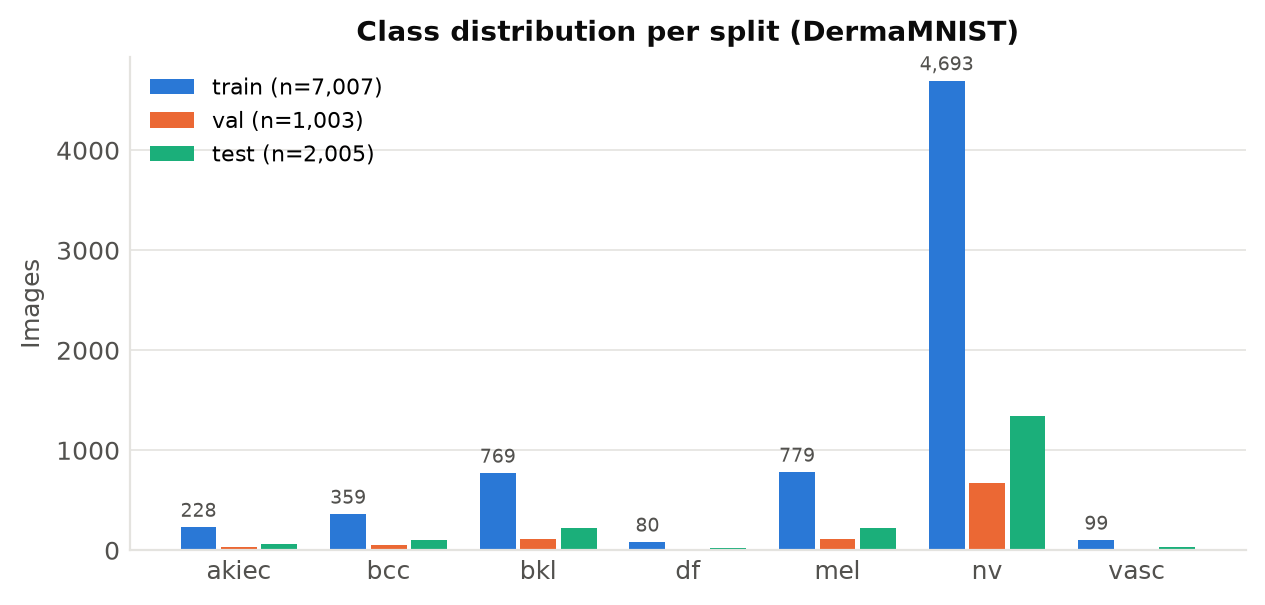
\includegraphics[width=0.82\textwidth]{../results/figures/eda_class_distribution.png}
\caption{Images per class and split. The \texttt{nv} class dominates every split; \texttt{df} and
\texttt{vasc} have fewer than 30 test images each.}
\label{fig:classdist}
\end{figure}

\textbf{Consequences for modelling.} (i)~A classifier that always answers \texttt{nv} already scores
\MajorityAcc\% test accuracy but a macro-F1 of only 0.11, so accuracy cannot be the selection metric; we select
on validation \emph{macro-F1}. (ii)~Rare classes need explicit help, so we use inverse-frequency class weights
in the loss (ablated in Section~\ref{sec:ablation}). (iii)~With 23--29 test images, per-class scores for
\texttt{df} and \texttt{vasc} carry wide uncertainty, so we report bootstrap confidence intervals.

\subsection{Visual inspection}
Figure~\ref{fig:samples} shows random training images. They vary a lot in illumination, zoom and skin tone.
Typical acquisition artefacts are dark circular \emph{vignetting} from the dermatoscope lens, hairs and
occasional reference objects in the field of view (e.g.\ in one \texttt{df} image). The classes overlap visually: many \texttt{mel}, \texttt{nv} and
\texttt{bkl} lesions are brown, roughly round pigmented blobs, and they differ mainly in fine texture, border
irregularity and colour variegation. Vascular lesions (\texttt{vasc}) stand out by their red/purple hue. The
lesion is almost always centred, and orientation is arbitrary. This motivates flip and 90\textdegree-rotation
augmentation, which leaves the label unchanged.

\begin{figure}[H]
\centering
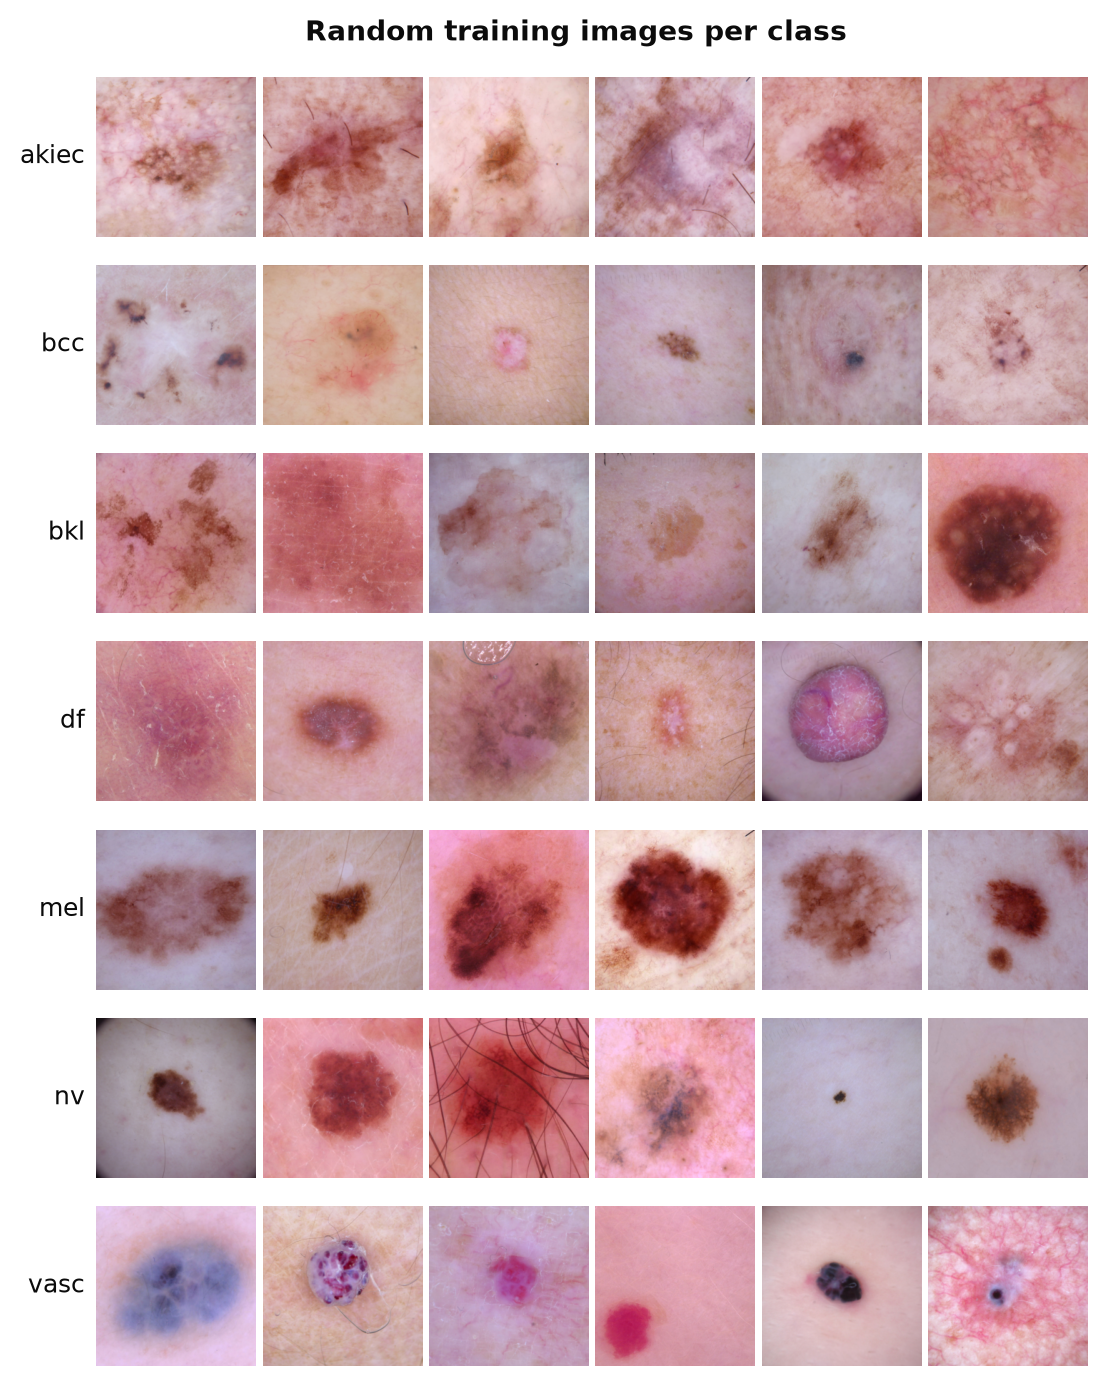
\includegraphics[width=0.70\textwidth]{../results/figures/eda_samples.png}
\caption{Six random training images per class (rows). Note vignetting, hairs and the strong visual similarity
of \texttt{mel}, \texttt{nv} and \texttt{bkl}.}
\label{fig:samples}
\end{figure}

\subsection{Colour statistics}
Over the training split, the per-channel mean (R, G, B) is (0.763, 0.538, 0.562) and the standard deviation is
(0.137, 0.159, 0.177). The images are red-dominant skin tones, quite unlike the ImageNet statistics
(0.485, 0.456, 0.406), which is one aspect of the \emph{domain shift} that fine-tuning has to bridge. We still
normalise with the ImageNet statistics, because the pretrained filters expect inputs on that scale.
Figure~\ref{fig:colour} shows that colour carries class information. Melanoma and benign keratoses are the
darkest classes (median luminance 0.584 and 0.592), while basal cell carcinoma is the brightest (0.668);
\texttt{vasc} and \texttt{bcc} have the highest blue component. The per-class mean images
(Figure~\ref{fig:meanimg}) confirm that lesions are centred. The pigmented classes (\texttt{mel},
\texttt{nv}, \texttt{bkl}) have a dark brown centre, and the \texttt{mel} blob is the darkest and widest.
\texttt{akiec}, \texttt{bcc} and \texttt{df} are only faintly pink, being less pigmented, and \texttt{vasc}
has a distinctly purple centre. Because colour is informative but also depends on the acquisition device, we use only \emph{mild}
colour jitter (Section~\ref{sec:workflow}). Strong jitter could erase real diagnostic cues.

\begin{figure}[H]
\centering
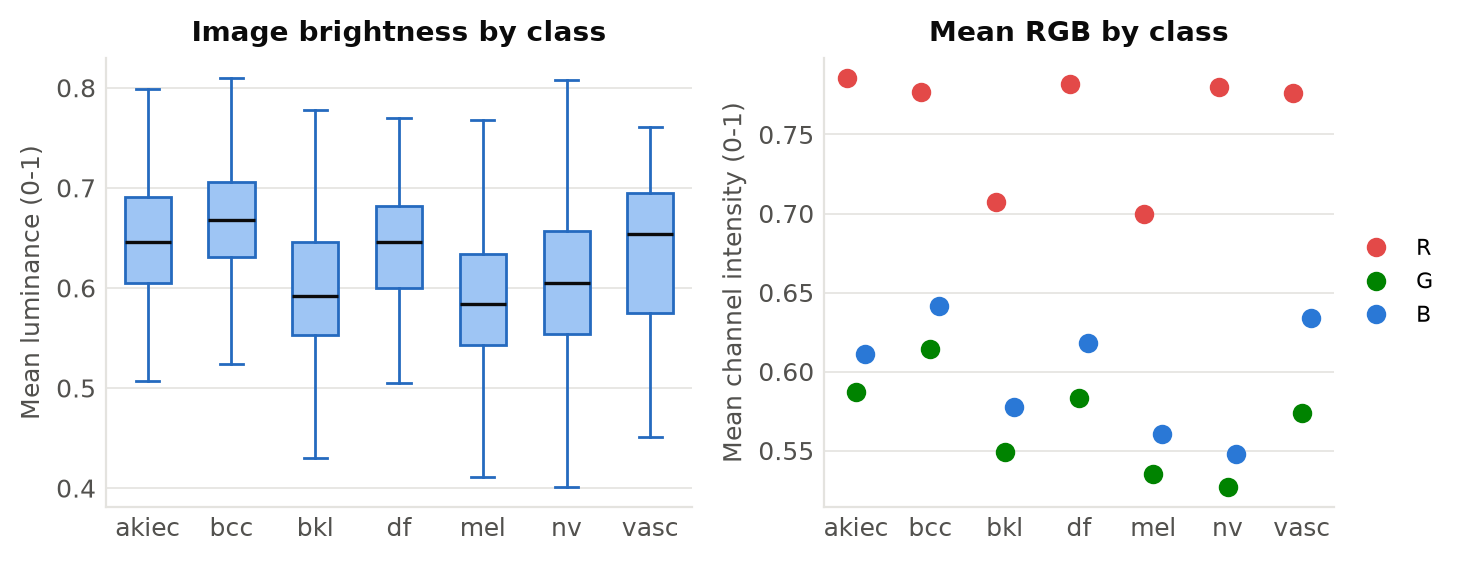
\includegraphics[width=0.92\textwidth]{../results/figures/eda_colour_stats.png}
\caption{Left: distribution of per-image mean luminance by class (boxes = IQR, whiskers = 1.5\,IQR).
Right: mean R, G, B intensity by class.}
\label{fig:colour}
\end{figure}

\begin{figure}[H]
\centering
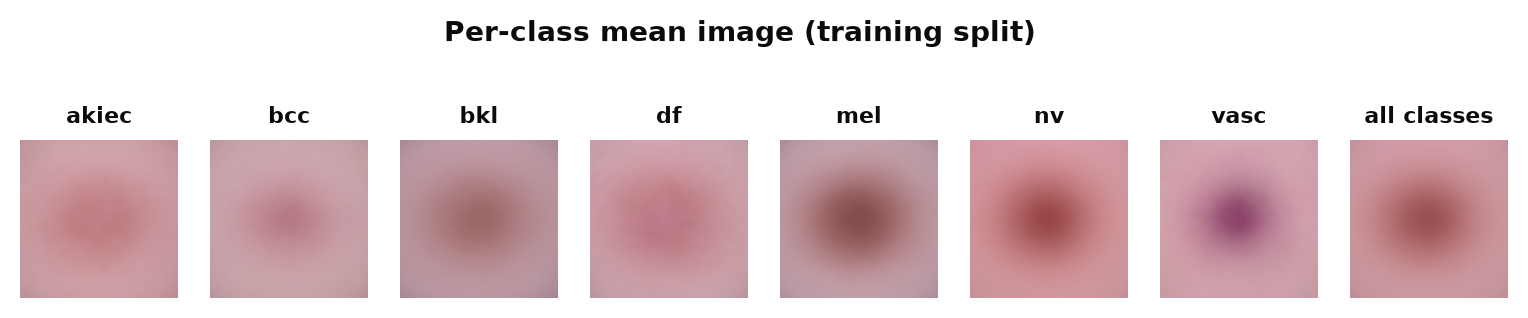
\includegraphics[width=0.98\textwidth]{../results/figures/eda_mean_images.png}
\caption{Pixel-wise mean image per class (training split). Lesions are centred; pigmented classes have a
brown centre (darkest and widest for \texttt{mel}), and \texttt{vasc} a purple one.}
\label{fig:meanimg}
\end{figure}

\subsection{Split integrity: duplicate and leakage audit}
\label{sec:leakage}
HAM10000 often contains \emph{several images of the same lesion}~\cite{ham10000}, and the DermaMNIST split is made
per image, not per lesion. Lesion identifiers are not distributed with DermaMNIST, so we audited the splits
directly in two ways:
\begin{enumerate}
  \item \textbf{Exact duplicates} (MD5 of raw pixels): \textbf{none} of the validation or test images is a
        byte-identical copy of a training image.
  \item \textbf{Near duplicates}: a 64-bit difference hash (dHash) of each image, then the Hamming distance to
        the nearest training image (Table~\ref{tab:dhash}).
\end{enumerate}

\begin{table}[H]
\centering
\caption{Near-duplicate audit with a 64-bit dHash. ``Label agreement'' is the share of pairs whose nearest
training image has the same diagnosis; the last row is the base rate over all images.}
\label{tab:dhash}
\small
\begin{tabular}{lrrrr}
\toprule
 & \multicolumn{2}{c}{Validation (n = 1{,}003)} & \multicolumn{2}{c}{Test (n = 2{,}005)} \\
\cmidrule(lr){2-3}\cmidrule(lr){4-5}
Distance to nearest train image & pairs & label agreement & pairs & label agreement \\
\midrule
$d = 0$ & 3 & 100\% & 3 & 100\% \\
$d \le 2$ & 15 & 73.3\% & 29 & 69.0\% \\
$d \le 4$ & 63 & 60.3\% & 122 & 70.5\% \\
any $d$ (base rate) & 1{,}003 & 56.0\% & 2{,}005 & 59.2\% \\
\bottomrule
\end{tabular}
\end{table}

The pairs at $d=0$ always share the label. Figure~\ref{fig:neardup} confirms that several of the closest pairs
are the same lesion photographed twice, with a slightly different shift or zoom. For $d \le 4$, though, label
agreement (60--71\%) is barely above the base rate (56--59\%). Coarse dHash therefore mostly finds
\emph{look-alike} lesions (round brown blobs on pink skin), not re-photographs. Our conclusion: a \emph{small}
amount of same-lesion leakage does exist between the official splits, so test scores may be slightly optimistic.
It cannot be measured exactly without lesion IDs. We keep the official split so that our numbers stay comparable
with published DermaMNIST results, and we list this as a limitation (Section~\ref{sec:limitations}).

\begin{figure}[H]
\centering
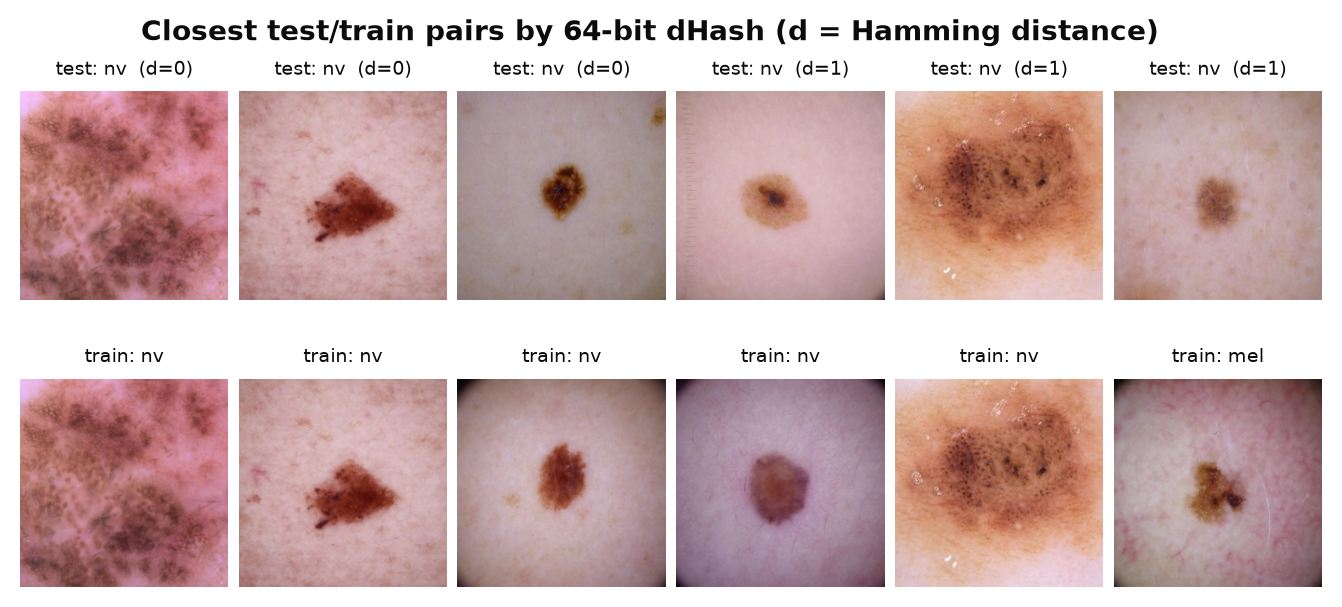
\includegraphics[width=0.85\textwidth]{../results/figures/eda_near_duplicates.png}
\caption{The six test images with the closest training image by dHash (top: test, bottom: nearest train image).
Pairs 1, 2 and 5 are the same lesion re-photographed; pairs 3, 4 and 6 are different lesions.}
\label{fig:neardup}
\end{figure}

\subsection{Summary of data-analysis findings}
\begin{itemize}
  \item Severe imbalance (58.7\,:\,1). We use macro-F1 for model selection and class-weighted loss for training.
  \item Arbitrary lesion orientation. We augment with flips and 90\textdegree{} rotations; the test-time version
        of this becomes 8-view TTA.
  \item Colour is informative but depends on the device. We use only mild colour jitter.
  \item Strong domain shift from ImageNet (colour statistics, texture-dominated content). Full fine-tuning
        should beat frozen features (tested in Section~\ref{sec:performance}).
  \item Small, partly measurable same-lesion leakage in the official splits. We keep it in mind when
        interpreting results.
\end{itemize}

\section{Workflow}
\label{sec:workflow}

Figure~\ref{fig:workflow} shows the end-to-end pipeline. Each box maps to one script in the codebase, so
the whole study can be re-run with \texttt{bash scripts/run\_all.sh}.

\begin{figure}[H]
\centering
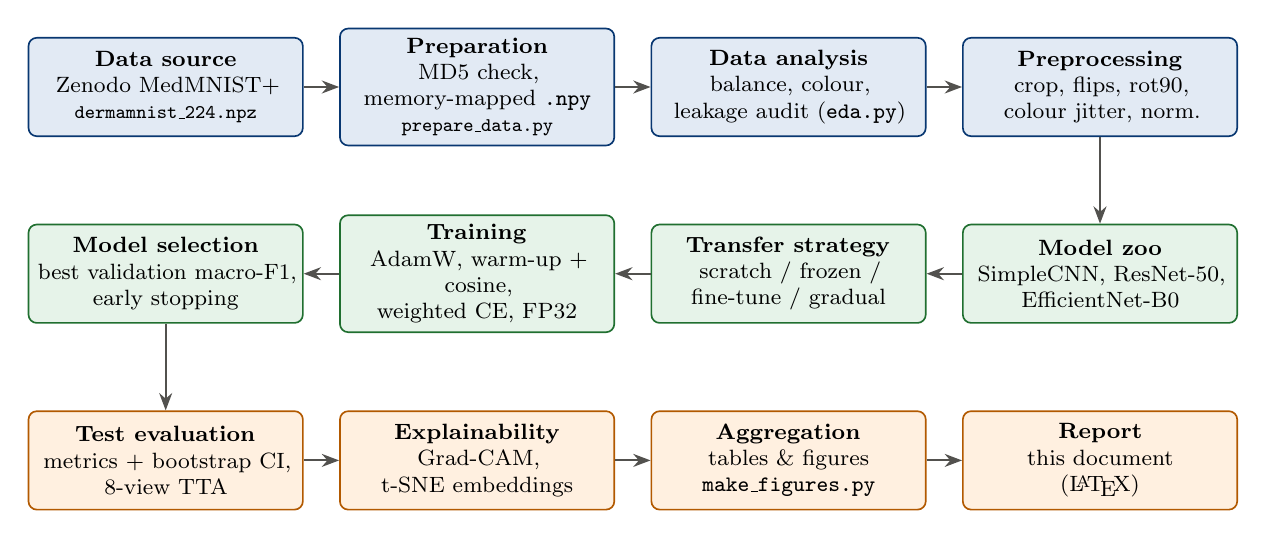
\begin{tikzpicture}[
  node distance=0.55cm and 0.45cm,
  box/.style={draw=#1!70!black, fill=#1!12, rounded corners=3pt, minimum height=1.25cm,
              text width=3.25cm, align=flush center, font=\footnotesize, line width=0.6pt},
  box/.default=diublue,
  arr/.style={-{Stealth[length=2.2mm]}, line width=0.7pt, color=ink2},
  lab/.style={font=\scriptsize\itshape, color=ink2}]
  % row 1: data
  \node[box] (src) {\textbf{Data source}\\ Zenodo MedMNIST+\\ {\scriptsize\texttt{dermamnist\_224.npz}}};
  \node[box, right=of src] (prep) {\textbf{Preparation}\\ MD5 check, memory-mapped \texttt{.npy}\\ {\scriptsize\texttt{prepare\_data.py}}};
  \node[box, right=of prep] (eda) {\textbf{Data analysis}\\ balance, colour,\\ leakage audit (\texttt{eda.py})};
  \node[box, right=of eda] (aug) {\textbf{Preprocessing}\\ crop, flips, rot90,\\ colour jitter, norm.};
  % row 2: modelling
  \node[box=diugreen, below=1.1cm of aug] (models) {\textbf{Model zoo}\\ SimpleCNN, ResNet-50,\\ EfficientNet-B0};
  \node[box=diugreen, left=of models] (strat) {\textbf{Transfer strategy}\\ scratch / frozen /\\ fine-tune / gradual};
  \node[box=diugreen, left=of strat] (train) {\textbf{Training}\\ AdamW, warm-up + cosine,\\ weighted CE, FP32};
  \node[box=diugreen, left=of train] (select) {\textbf{Model selection}\\ best validation macro-F1, early stopping};
  % row 3: evaluation
  \node[box=orange, below=1.1cm of select] (eval) {\textbf{Test evaluation}\\ metrics + bootstrap CI,\\ 8-view TTA};
  \node[box=orange, right=of eval] (explain) {\textbf{Explainability}\\ Grad-CAM,\\ t-SNE embeddings};
  \node[box=orange, right=of explain] (figs) {\textbf{Aggregation}\\ tables \& figures\\ \texttt{make\_figures.py}};
  \node[box=orange, right=of figs] (report) {\textbf{Report}\\ this document\\ (\LaTeX)};
  \draw[arr] (src) -- (prep);
  \draw[arr] (prep) -- (eda);
  \draw[arr] (eda) -- (aug);
  \draw[arr] (aug) -- (models);
  \draw[arr] (models) -- (strat);
  \draw[arr] (strat) -- (train);
  \draw[arr] (train) -- (select);
  \draw[arr] (select) -- (eval);
  \draw[arr] (eval) -- (explain);
  \draw[arr] (explain) -- (figs);
  \draw[arr] (figs) -- (report);
\end{tikzpicture}
\caption{End-to-end workflow. Blue: data stages; green: modelling and training; orange: evaluation and
reporting. The test split is used only in the orange stages, after a checkpoint has been chosen on the
validation split.}
\label{fig:workflow}
\end{figure}

\subsection{Step-by-step description}
\begin{enumerate}[leftmargin=1.4em]
  \item \textbf{Acquisition.} The 224$\times$224 DermaMNIST archive (\DatasetSizeMB\,MB) is downloaded from the
        MedMNIST+ Zenodo record and checked with an MD5 checksum.
  \item \textbf{Preparation.} The three official splits are written as separate \texttt{.npy} files and
        \emph{memory-mapped}, so the 1.5\,GB uint8 tensor is never fully loaded into RAM. This matters on the
        16\,GB development machine.
  \item \textbf{Data analysis} (Section~\ref{sec:data}). Class counts, colour statistics, mean images, and
        exact and near-duplicate checks between splits.
  \item \textbf{Preprocessing and augmentation.} Training images go through
        \texttt{RandomResizedCrop}(224, scale 0.75--1.0), horizontal and vertical flips, random multiples of
        90\textdegree{} rotation (dermatoscopic images have no canonical orientation), mild colour jitter
        (brightness/contrast 0.2, saturation 0.15, hue 0.02) and ImageNet mean/std normalisation. Validation and
        test images are only normalised.
  \item \textbf{Training} (Section~\ref{sec:modeling}). Every configuration uses AdamW, a one-epoch linear
        warm-up followed by cosine decay, FP32 arithmetic (Section~\ref{sec:modeling} explains why not FP16), gradient
        clipping at norm 5 and class-weighted cross-entropy with label smoothing 0.05.
  \item \textbf{Model selection.} After each epoch the model is scored on the validation split. The checkpoint
        with the highest \emph{validation macro-F1} is kept, and training stops early if there is no improvement
        for 6 epochs (8 for the scratch baseline).
  \item \textbf{Evaluation} (Section~\ref{sec:performance}). The selected checkpoint is scored once on the test
        split, with and without 8-view dihedral TTA. Metrics come with 1{,}000-resample bootstrap confidence
        intervals.
  \item \textbf{Explainability.} Grad-CAM heat-maps and t-SNE plots of the penultimate-layer embeddings, for the
        best model.
\end{enumerate}

\subsection{Experimental environment}
\begin{table}[H]
\centering
\caption{Hardware and software used for every experiment.}
\label{tab:env}
\small
\begin{tabularx}{\textwidth}{lX}
\toprule
GPU & NVIDIA GeForce GTX 1660 SUPER, 6\,GB GDDR6 (Turing, no tensor cores) \\
CPU / RAM & AMD Ryzen 5 5500 (6 cores / 12 threads) / 16\,GB \\
OS & Ubuntu 26.04 LTS, NVIDIA driver 595.91 \\
Software & Python 3.12, PyTorch~\cite{pytorch} \TorchVersion{} (CUDA 12.6), torchvision 0.29.1, scikit-learn 1.9.1 \\
Seeding & global seed 42 for Python, NumPy and PyTorch (cuDNN autotuning on, so not bit-exact) \\
\bottomrule
\end{tabularx}
\end{table}

\section{Modelling}
\label{sec:modeling}

\subsection{Architectures}

\paragraph{Baseline: SimpleCNN trained from scratch.} A VGG-style network~\cite{vgg} with five blocks. Each
block has two $3\times3$ convolution--BatchNorm--ReLU layers followed by $2\times2$ max-pooling, with widths
16-32-64-128-256. Global average pooling, dropout ($p=0.3$) and a linear layer produce the 7 logits. It has
\textbf{1.18\,M} parameters, all randomly initialised (PyTorch default Kaiming-uniform). This baseline shows what is achievable
\emph{without} transfer learning.

\paragraph{ResNet-50~\cite{resnet}.} A 50-layer residual network with bottleneck blocks arranged in four stages
(\texttt{layer1}--\texttt{layer4}, output stride 32), followed by global average pooling. We use the torchvision
\texttt{IMAGENET1K\_V2} weights (80.86\% ImageNet top-1, 4.09\,GFLOPs). The 1000-way classifier is replaced by
dropout ($p=0.3$) and a $2048\to7$ linear layer, giving \textbf{23.52\,M} parameters.

\paragraph{EfficientNet-B0~\cite{efficientnet}.} A compound-scaled network built from inverted-residual MBConv
blocks with squeeze-and-excitation and SiLU activations. We use torchvision \texttt{IMAGENET1K\_V1} weights
(77.69\% ImageNet top-1, 0.39\,GFLOPs, about 10$\times$ cheaper than ResNet-50). The head is again dropout
followed by a $1280\to7$ linear layer, giving \textbf{4.02\,M} parameters.

\subsection{Transfer-learning strategies}
Let $f_\theta$ be the pretrained backbone and $g_\phi$ the new classification head. We compare:

\begin{enumerate}
  \item \textbf{Scratch} (baseline only): $\theta,\phi$ randomly initialised, all trained with learning rate
        $10^{-3}$.
  \item \textbf{Feature extraction (frozen backbone).} $\theta$ is fixed at its ImageNet values and BatchNorm is
        kept in inference mode (running statistics are not updated). Only $g_\phi$ is trained, with learning
        rate $10^{-3}$. This is the cheapest option: no gradients flow through the backbone.
  \item \textbf{Full fine-tuning with discriminative learning rates.} All parameters are trained, but the
        backbone uses a $10\times$ smaller learning rate ($\eta_\theta = 10^{-4}$) than the randomly initialised
        head ($\eta_\phi = 10^{-3}$). The new head can adapt fast while the pretrained features are only
        gently adjusted, which limits catastrophic forgetting.
  \item \textbf{Gradual unfreezing} (ULMFiT-style~\cite{ulmfit}). Training starts with the head only, and one
        backbone stage is unfrozen every two epochs, from the output side inwards (Table~\ref{tab:gradual}).
        Each stage nearer the input gets half the learning rate of the stage above it, because early layers
        hold generic edge and colour detectors that need little change~\cite{yosinski2014}.
\end{enumerate}

\begin{table}[H]
\centering
\caption{Gradual-unfreezing schedule for ResNet-50 (12 epochs).}
\label{tab:gradual}
\begin{tabular}{llrr}
\toprule
Epochs & Trainable modules & Peak LR of newest stage & Trainable params \\
\midrule
1--2 & head & $10^{-3}$ (head) & 14\,K \\
3--4 & + \texttt{layer4} & $1.0\times10^{-4}$ & 14.98\,M \\
5--6 & + \texttt{layer3} & $5.0\times10^{-5}$ & 22.08\,M \\
7--8 & + \texttt{layer2} & $2.5\times10^{-5}$ & 23.30\,M \\
9--12 & + stem, \texttt{layer1} & $1.25\times10^{-5}$ & 23.52\,M \\
\bottomrule
\end{tabular}
\end{table}

\subsection{Loss function and class imbalance}
We minimise class-weighted cross-entropy with label smoothing~\cite{labelsmoothing} $\varepsilon = 0.05$:
\begin{equation}
\mathcal{L} = \frac{1}{\sum_i w_{y_i}}\sum_{i}\Big[(1-\varepsilon)\,w_{y_i}\big(-\log p_{i,y_i}\big)
 + \frac{\varepsilon}{K}\sum_{c=1}^{K} w_c\big(-\log p_{i,c}\big)\Big],
\end{equation}
where $p_{i,c}$ is the softmax probability of class $c$ for image $i$ and $K=7$ (this is exactly PyTorch's
\texttt{CrossEntropyLoss(weight=w, label\_smoothing=$\varepsilon$)}). The class weights are the \emph{square root} of the
inverse class frequency, rescaled to mean 1:
\begin{equation}
w_c \propto \Big(\frac{N}{K\,n_c}\Big)^{1/2}.
\end{equation}
Full inverse-frequency weighting would weight \texttt{df} 59 times more than \texttt{nv}; with only 80
\texttt{df} images, that tends to overfit the rare classes. The square root is a milder compromise. The
resulting weights are
\texttt{akiec} 1.11, \texttt{bcc} 0.88, \texttt{bkl} 0.60, \texttt{df} 1.87, \texttt{mel} 0.60,
\texttt{nv} 0.24, \texttt{vasc} 1.68. Section~\ref{sec:ablation} compares this with unweighted cross-entropy.

\subsection{Optimisation}
We use AdamW~\cite{adamw} ($\beta=(0.9, 0.999)$, weight decay $10^{-4}$) with a batch size of 32. The learning
rate rises linearly over the first epoch (warm-up) and then follows a cosine decay to zero~\cite{sgdr}:
\begin{equation}
\eta_t = \eta_{\max}\cdot \tfrac12\Big(1+\cos\big(\pi\,\tfrac{t - t_w}{T - t_w}\big)\Big), \quad t \ge t_w .
\end{equation}
Gradients are clipped to an $\ell_2$ norm of 5. We trained in FP32. Our benchmark showed FP16 autocast to be
3.3$\times$ \emph{slower} on this GPU (34 vs 112 img/s for ResNet-50), because the GTX 16-series has no tensor
cores. Mixed precision is still available in the code (\texttt{--amp}) for tensor-core GPUs.

\begin{table}[H]
\centering
\caption{Configuration of the seven experiments. All share the data pipeline, the loss (unless stated),
AdamW, warm-up + cosine schedule, batch size 32 and seed 42.}
\label{tab:runs}
\footnotesize
\setlength{\tabcolsep}{4pt}
\begin{tabular}{llllrlll}
\toprule
ID & Run name (code) & Backbone & Strategy & Ep. & LR head & LR backbone & Loss \\
\midrule
E1 & \texttt{scratch\_cnn} & SimpleCNN & scratch & 30 & $10^{-3}$ & (all layers $10^{-3}$) & weighted CE \\
E2 & \texttt{resnet50\_frozen} & ResNet-50 & frozen & 10 & $10^{-3}$ & frozen & weighted CE \\
E3 & \texttt{effnetb0\_frozen} & EffNet-B0 & frozen & 10 & $10^{-3}$ & frozen & weighted CE \\
E4 & \texttt{resnet50\_finetune} & ResNet-50 & fine-tune & 12 & $10^{-3}$ & $10^{-4}$ & weighted CE \\
E5 & \texttt{effnetb0\_finetune} & EffNet-B0 & fine-tune & 12 & $10^{-3}$ & $10^{-4}$ & weighted CE \\
E6 & \texttt{resnet50\_gradual} & ResNet-50 & gradual & 12 & $10^{-3}$ & $10^{-4}\!\to\!1.25{\cdot}10^{-5}$ & weighted CE \\
E7 & \texttt{resnet50\_finetune\_noweights} & ResNet-50 & fine-tune & 12 & $10^{-3}$ & $10^{-4}$ & plain CE \\
\bottomrule
\end{tabular}
\end{table}

\paragraph{Model selection and early stopping.} After every epoch we compute validation macro-F1 and keep the
checkpoint with the best value. Training stops when there has been no improvement for 6 epochs (8 for E1).
The test split is never used for any decision; it is evaluated once per run, at the end.

\section{Performance Evaluation}
\label{sec:performance}

\subsection{Evaluation protocol and metrics}
Each run is evaluated once on the 2{,}005-image test split, using the checkpoint chosen on validation
macro-F1. With $\mathrm{TP}_c$, $\mathrm{FP}_c$, $\mathrm{FN}_c$ counted one-vs-rest for each class $c$:
\begin{itemize}
  \item \textbf{Accuracy}: fraction of correct predictions. This is the official MedMNIST metric, but it is
        dominated by \texttt{nv}.
  \item \textbf{Balanced accuracy}: mean per-class recall,
        $\frac1K\sum_c \mathrm{TP}_c/(\mathrm{TP}_c+\mathrm{FN}_c)$.
  \item \textbf{Macro-F1} (primary): unweighted mean of per-class
        $F_1 = 2\,\mathrm{P}_c\mathrm{R}_c/(\mathrm{P}_c+\mathrm{R}_c)$. Every class counts equally, including
        melanoma and the rare classes.
  \item \textbf{Macro AUC}: mean one-vs-rest area under the ROC curve. It is threshold-free and is the second
        official MedMNIST metric.
  \item \textbf{Expected calibration error (ECE)}~\cite{guo2017}: with 15 equal-width confidence bins $B_m$,
        $\mathrm{ECE} = \sum_m \frac{|B_m|}{n}\,\big|\mathrm{acc}(B_m) - \mathrm{conf}(B_m)\big|$. Lower is better.
        This matters when predicted probabilities are used for triage.
  \item \textbf{95\% confidence intervals}: percentile bootstrap over 1{,}000 resamples of the test set.
\end{itemize}
\textbf{Test-time augmentation (TTA)} averages the softmax outputs over the 8 dihedral transforms of each
image (4 rotations $\times$ \{identity, horizontal flip\}). These are exactly the symmetries the model saw
during training. Whether the best model uses TTA is also decided on the validation split.


\subsection{Training dynamics}
Figure~\ref{fig:curves} (left) shows validation macro-F1 per epoch for all seven runs. Three regimes are
visible:
\begin{itemize}
  \item \textbf{Scratch.} The SimpleCNN learns slowly and noisily, climbing from 0.20 to its best value of 0.49 at
        epoch~\ScratchBestEpoch, then plateauing. Early stopping ended it at epoch 27.
  \item \textbf{Frozen backbones} plateau within about five epochs at 0.55 (ResNet-50) and 0.59 (EfficientNet-B0).
        A linear head on fixed ImageNet features has little capacity to adapt to dermatoscopic texture.
  \item \textbf{Fine-tuned backbones} pass 0.70 by epoch 3--4 and keep improving, with ResNet-50 reaching 0.795 at
        epoch \RFineBestEpoch.
\end{itemize}
Epoch-to-epoch swings of $\pm0.03$--$0.05$ are expected. The validation split has only 12 \texttt{df} and 14
\texttt{vasc} images, so a single image changes that class's recall by 7--8 points.

The loss curves of the selected model (Figure~\ref{fig:curves}, right) show no overfitting within 12 epochs: the
validation loss keeps falling until the selected epoch. The training loss stays \emph{above} the validation loss
because it is measured under augmentation, dropout, label smoothing and class weighting. The validation loss is
plain cross-entropy on clean images, so the two curves are not on the same scale.

\begin{figure}[H]
\centering
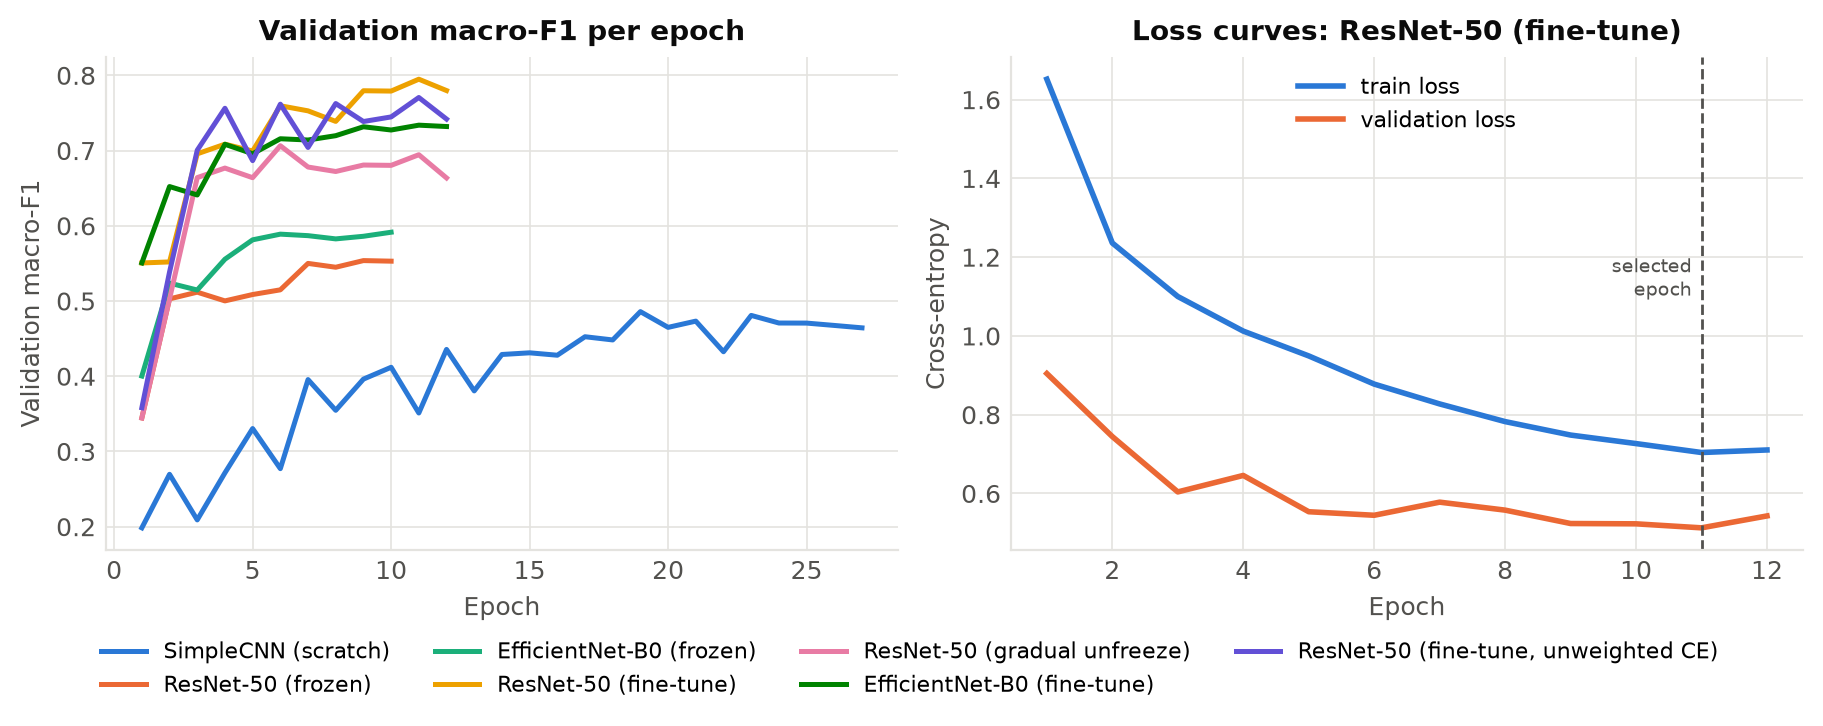
\includegraphics[width=\textwidth]{../results/figures/training_curves.png}
\caption{Left: validation macro-F1 per epoch for all runs. Right: training and validation loss of the selected
model (ResNet-50, full fine-tuning); the dashed line marks the checkpoint chosen on validation macro-F1.}
\label{fig:curves}
\end{figure}

\subsection{Main results}
Table~\ref{tab:results} and Figure~\ref{fig:comparison} summarise the test results (single view, i.e.\ without
TTA, so every run is compared on equal terms).

\begin{table}[H]
\centering
\caption{Test-set results of all runs (single view). Val F1 is the validation macro-F1 of the selected
checkpoint; macro-F1 is shown with its 95\% bootstrap CI. Bold: the model selected on validation.
Acc.\ = accuracy, Bal.\ = balanced accuracy, both in \%.}
\label{tab:results}
\footnotesize
\setlength{\tabcolsep}{3.5pt}
\resizebox{\textwidth}{!}{%
\begin{tabular}{lrrcrrrlrr}
\toprule
Run & Params & Trainable & Best ep. & Val F1 & Acc. & Bal. & Macro-F1 [95\% CI] & AUC & ECE \\
 & (M) & (M) & / run & (\%) & (\%) & (\%) & (\%) & & \\
\midrule
\inputrows{generated/results_table.tex}
\midrule
\multicolumn{5}{l}{Majority class (always \texttt{nv})} & \MajorityAcc & 14.3 & 11.5 & 0.500 & -- \\
\bottomrule
\end{tabular}}
\end{table}

\begin{figure}[H]
\centering
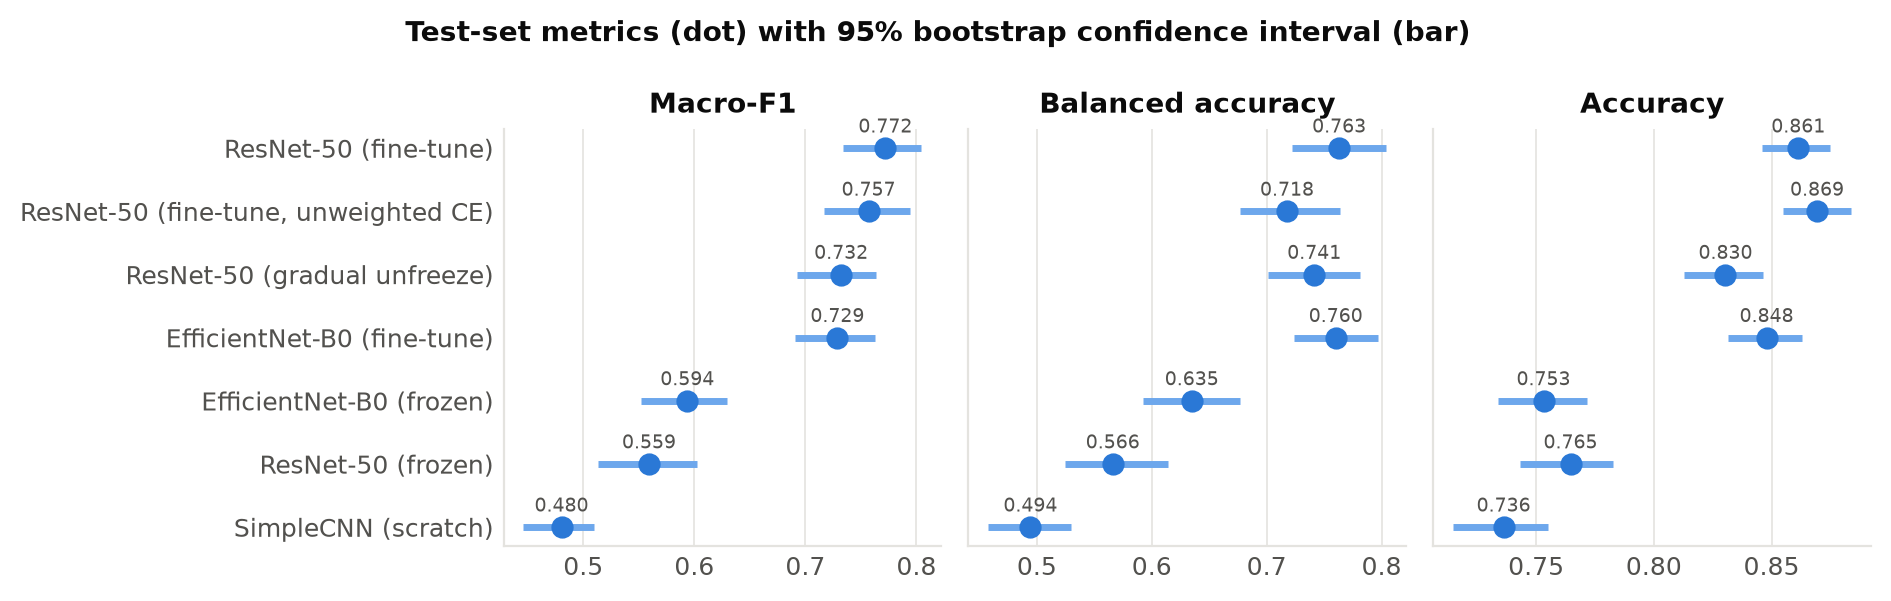
\includegraphics[width=\textwidth]{../results/figures/test_metric_comparison.png}
\caption{Test macro-F1, balanced accuracy and accuracy with 95\% bootstrap confidence intervals, sorted by
macro-F1.}
\label{fig:comparison}
\end{figure}

\paragraph{Finding 1: transfer learning is decisive.} The from-scratch SimpleCNN reaches \ScratchAcc\% accuracy,
only 6.7 points above the trivial majority classifier, and a macro-F1 of just \ScratchFOne\%. It never correctly
detects a single dermatofibroma (\texttt{df} F1 = \ScratchFOneDf). Fine-tuning an ImageNet ResNet-50 raises
macro-F1 to \RFineFOne\% (+29.2 points) and accuracy to \RFineAcc\%. The 95\% CIs, \RFineFOneCI{} against
\ScratchFOneCI{}, are far apart, so the gain is not a sampling artefact. With only 80--100 training images for the
rarest classes, features learned from 1.28\,M natural images~\cite{imagenet} give a far better starting point than
random initialisation.

\paragraph{Finding 2: frozen features are not enough; the domain shift has to be bridged.} Feature extraction
improves on scratch training (macro-F1 \RFrozenFOne\% for ResNet-50, \EFrozenFOne\% for EfficientNet-B0), but
full fine-tuning adds another \textbf{+21.3} (ResNet-50) and \textbf{+13.5} (EfficientNet-B0) points. This matches
the colour and texture shift found in Section~\ref{sec:data}. Dermatoscopic images look nothing like ImageNet
photographs, so the mid- and high-level filters must change, not just the classifier on top. The same pattern has
been reported for other medical-imaging transfer problems~\cite{raghu2019}.

\paragraph{Finding 3: ResNet-50 is the most accurate, EfficientNet-B0 the most efficient.} When frozen,
EfficientNet-B0 transfers better (\EFrozenFOne\% vs \RFrozenFOne\% macro-F1). After fine-tuning, ResNet-50 leads on
macro-F1 (\RFineFOne\% vs \EFineFOne\%) and accuracy (\RFineAcc\% vs \EFineAcc\%), while EfficientNet-B0 has a
slightly higher AUC (\EFineAUC{} vs \RFineAUC). EfficientNet-B0 does this with 5.9$\times$ fewer parameters,
10$\times$ fewer FLOPs and less than half the training time (\EFineTrainMin{} vs \RFineTrainMin\,min). It is the
better choice under a tight compute or deployment budget. The two macro-F1 CIs overlap (\EFineFOneCI{} vs
\RFineFOneCI), so the ResNet-50 lead is suggestive rather than conclusive.

\subsection{Effect of the transfer strategy: gradual unfreezing}
Gradual unfreezing reached \RGradFOne\% macro-F1, below full fine-tuning (\RFineFOne\%). Its best validation
epoch was epoch~\RGradBestEpoch, the end of the phase in which only \texttt{layer3}, \texttt{layer4} and the head
were trainable. Validation F1 did not improve after \texttt{layer2} and the stem were released. Two effects
explain this:
\begin{enumerate}
  \item the shared cosine schedule had already decayed the learning rate by then, so the lower stages, which
        start with $\le 2.5\times10^{-5}$, barely move;
  \item in a 12-epoch budget, half of the epochs are spent with most of the network frozen.
\end{enumerate}
The main purpose of gradual unfreezing is to protect pretrained features from large early gradients. In full
fine-tuning, warm-up and discriminative learning rates already provide that protection. Gradual unfreezing still
has advantages: it is about 30\% cheaper (\RGradTrainMin{} vs \RFineTrainMin\,min) and has the highest
single-view AUC among the class-weighted ResNet runs (\RGradAUC). With a longer budget, or with a separate
schedule restarted for each newly unfrozen stage, the gap would likely narrow.

\subsection{Ablation: class-weighted loss}
\label{sec:ablation}
Removing the class weights (E7 vs E4, everything else identical) shows a clear trade-off:

\begin{table}[H]
\centering
\caption{Class-weighted vs unweighted cross-entropy (ResNet-50, full fine-tuning, single view).}
\label{tab:ablation}
\small
\begin{tabular}{lrrrrrrr}
\toprule
Loss & Acc.\ (\%) & Bal.\ acc.\ (\%) & Macro-F1 (\%) & AUC & ECE & F1 \texttt{df} & F1 \texttt{vasc} \\
\midrule
weighted ($\sqrt{\text{inv.\ freq.}}$) & \RFineAcc & \textbf{\RFineBalAcc} & \textbf{\RFineFOne} & \RFineAUC & \RFineECE & \textbf{\RFineFOneDf} & \textbf{\RFineFOneVasc} \\
unweighted & \textbf{\RNoWAcc} & \RNoWBalAcc & \RNoWFOne & \textbf{\RNoWAUC} & \textbf{\RNoWECE} & \RNoWFOneDf & \RNoWFOneVasc \\
\bottomrule
\end{tabular}
\end{table}

Class weighting raises balanced accuracy by 4.5 points and macro-F1 by 1.5 points. The gain comes from the two
rarest classes (\texttt{df} +6.0 and \texttt{vasc} +5.3 F1 points). The cost is a little accuracy on the
majority classes (overall accuracy $-0.8$, \texttt{nv} F1 \RFineFOneNv{} vs \RNoWFOneNv) and much worse
calibration (ECE \RFineECE{} vs \RNoWECE). Weighting deliberately shifts probability mass towards rare classes,
so the raw softmax outputs no longer estimate true class frequencies. The unweighted model has the best AUC of
all runs (\RNoWAUC), so its \emph{ranking} of images is excellent. Its default arg-max decision rule simply
favours \texttt{nv}. In practice: if calibrated risk scores are needed, train unweighted and tune per-class
thresholds on validation; if balanced detection with a plain arg-max is needed, use weighting. The macro-F1
CIs overlap (\RFineFOneCI{} vs \RNoWFOneCI), so the macro-F1 difference is small relative to test-set noise.

\subsection{Test-time augmentation}
Averaging over the 8 dihedral views (Appendix, Table~\ref{tab:tta}) improves accuracy (+0.7 to +1.9 points) and
macro-AUC (+0.003 to +0.010) for \emph{every} run. It improves macro-F1 for six of the seven runs (+1.9 to +3.3
points; frozen EfficientNet-B0 is essentially unchanged at $-0.1$), at 8$\times$ the inference cost. For the selected model, TTA also
raised validation macro-F1 (0.795 $\rightarrow$ 0.810), so the final model uses TTA, a decision made on
validation only. Its final test performance is:

\begin{center}
\begin{tabular}{lll}
\toprule
\multicolumn{3}{c}{\textbf{Final model: ResNet-50, full fine-tuning, 8-view TTA (test set, n = 2{,}005)}} \\
\midrule
Accuracy & \textbf{\RFineAccTTA\%} & 95\% CI \RFineAccTTACI \\
Balanced accuracy & \textbf{\RFineBalAccTTA\%} & 95\% CI \RFineBalAccTTACI \\
Macro-F1 & \textbf{\RFineFOneTTA\%} & 95\% CI \RFineFOneTTACI \\
Macro AUC & \textbf{\RFineAUCTTA} & 95\% CI \RFineAUCTTACI \\
Cohen's $\kappa$ / ECE & \RFineKappaTTA{} / \RFineECETTA & \\
\bottomrule
\end{tabular}
\end{center}

\subsection{Per-class analysis of the final model}
\begin{table}[H]
\centering
\caption{Per-class test performance of the final model (ResNet-50 fine-tuned, 8-view TTA).}
\label{tab:perclass}
\begin{tabular}{lrrrrr}
\toprule
Class & Support & Precision (\%) & Recall (\%) & F1 (\%) & AUC \\
\midrule
\inputrows{generated/per_class_table.tex}
\bottomrule
\end{tabular}
\end{table}

\begin{figure}[H]
\centering
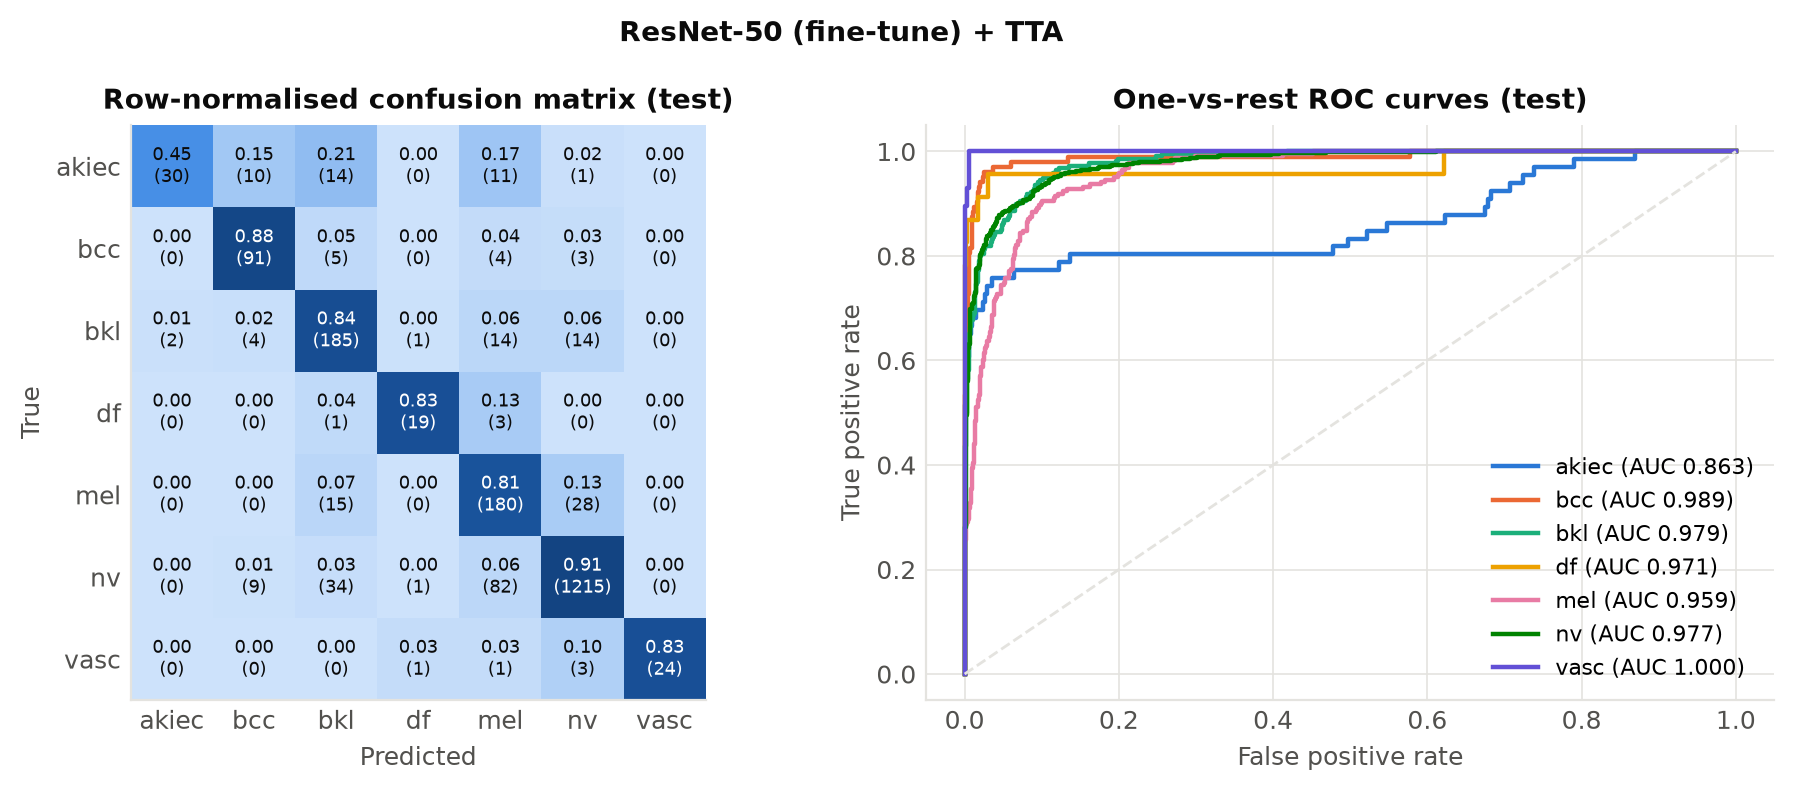
\includegraphics[width=\textwidth]{../results/figures/best_confusion_roc.png}
\caption{Final model on the test set: row-normalised confusion matrix (counts in brackets) and one-vs-rest ROC
curves.}
\label{fig:confusion}
\end{figure}

Table~\ref{tab:perclass} and Figure~\ref{fig:confusion} show where the model succeeds and fails.
\begin{itemize}
  \item \textbf{Strong classes.} \texttt{nv} (F1 \BestFOneNv\%), \texttt{vasc} (\BestFOneVasc\%, with 100\%
        precision), \texttt{df} (\BestFOneDf\%) and \texttt{bcc} (\BestFOneBcc\%). The visually distinctive
        \texttt{vasc} and \texttt{bcc} classes reach AUC \BestAUCVasc{} and \BestAUCBcc{}.
  \item \textbf{Melanoma} has recall \BestRecMel\% and precision \BestPrecMel\%. Of the 223 melanomas, 28 are
        called \texttt{nv} and 15 \texttt{bkl}. In the other direction, 82 nevi (6.1\% of all nevi) are flagged as
        melanoma, which accounts for most of its false positives. For a screening aid, this direction of error
        (over-calling melanoma rather than missing it) is the safer one.
  \item \textbf{Actinic keratoses (\texttt{akiec})} are the weakest class. When the model predicts \texttt{akiec}
        it is almost always right (precision \BestPrecAkiec\%), but it finds only \BestRecAkiec\% of them. Missed
        cases go to \texttt{bkl} (14), \texttt{mel} (11) and \texttt{bcc} (10). \texttt{akiec} and \texttt{bkl}
        are both scaly, keratinocytic lesions, and pigmented actinic keratoses can mimic melanoma. Its lower AUC
        (\BestAUCAkiec) shows that the class is hard to separate at any threshold, not only at the arg-max.
\end{itemize}

Figure~\ref{fig:heatmap} compares per-class F1 across all runs. Fine-tuning improves every class. The largest
gains are on \texttt{bcc} ($+0.29$ over frozen ResNet-50), \texttt{df} ($+0.36$) and \texttt{vasc} ($+0.30$),
the classes with the most distinctive local structure.

\begin{figure}[H]
\centering
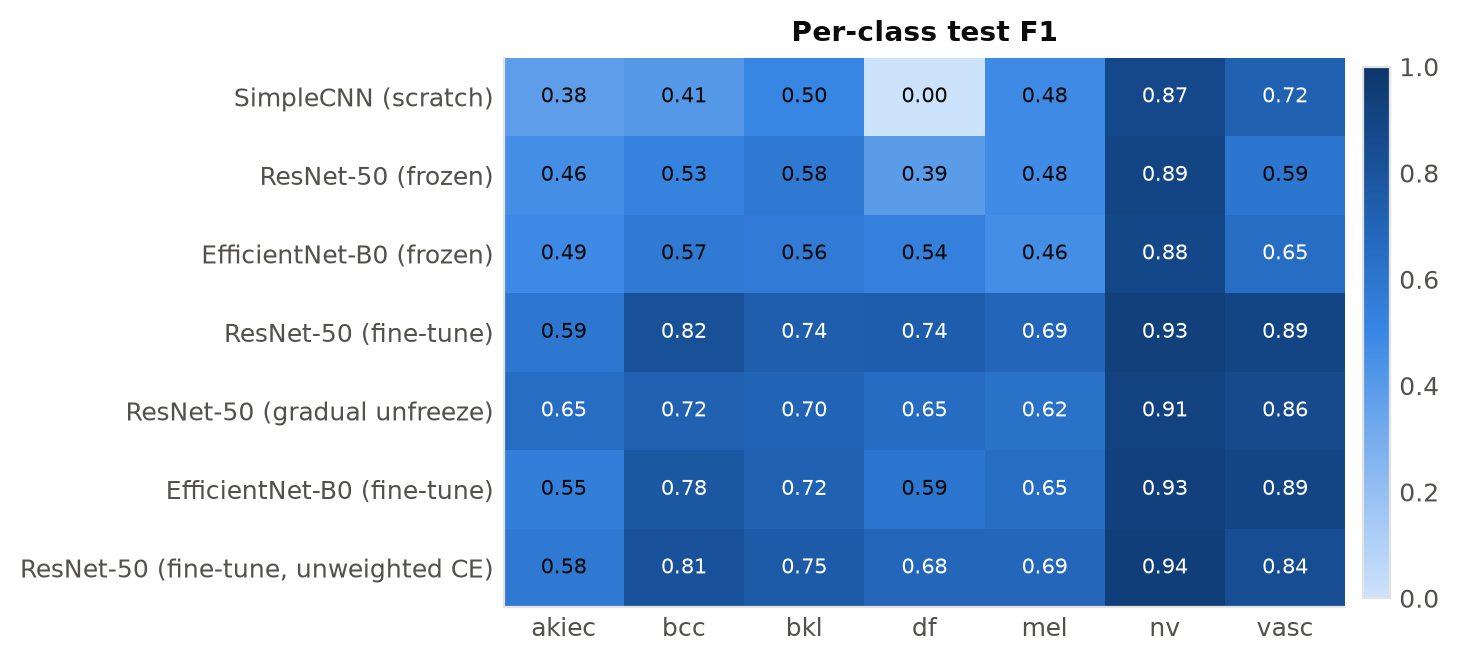
\includegraphics[width=0.85\textwidth]{../results/figures/per_class_f1_heatmap.png}
\caption{Per-class test F1 (single view) for every run.}
\label{fig:heatmap}
\end{figure}

\subsection{Calibration}
\begin{figure}[H]
\centering
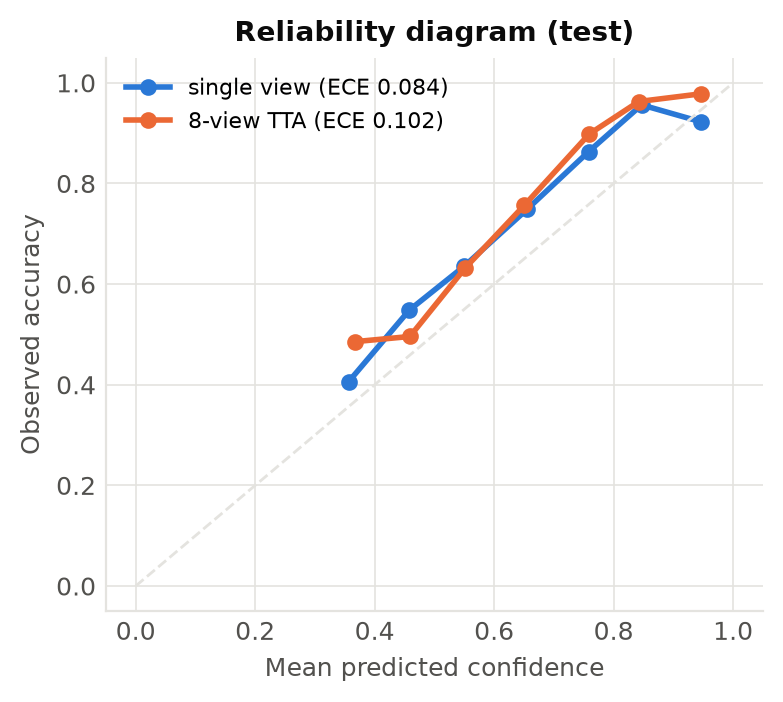
\includegraphics[width=0.42\textwidth]{../results/figures/best_reliability.png}
\caption{Reliability diagram of the final model (10 bins with at least 10 images). Points above the diagonal
indicate under-confidence.}
\label{fig:reliability}
\end{figure}
The reliability diagram (Figure~\ref{fig:reliability}) lies \emph{above} the diagonal: predictions made with
55--65\% confidence are correct 63--75\% of the time, so the model is \emph{under}-confident (ECE \RFineECE{} single
view, \RFineECETTA{} with TTA). The causes are label smoothing (which caps the target probability at 0.957),
class weighting (Section~\ref{sec:ablation}) and, for TTA, averaging over views, which further softens the
outputs. Ranking quality (AUC) is unaffected. If calibrated probabilities are needed, one temperature parameter
fitted on the validation split (temperature scaling~\cite{guo2017}) would correct this without changing any
prediction.

\subsection{Explainability: Grad-CAM and learned representations}
\begin{figure}[H]
\centering
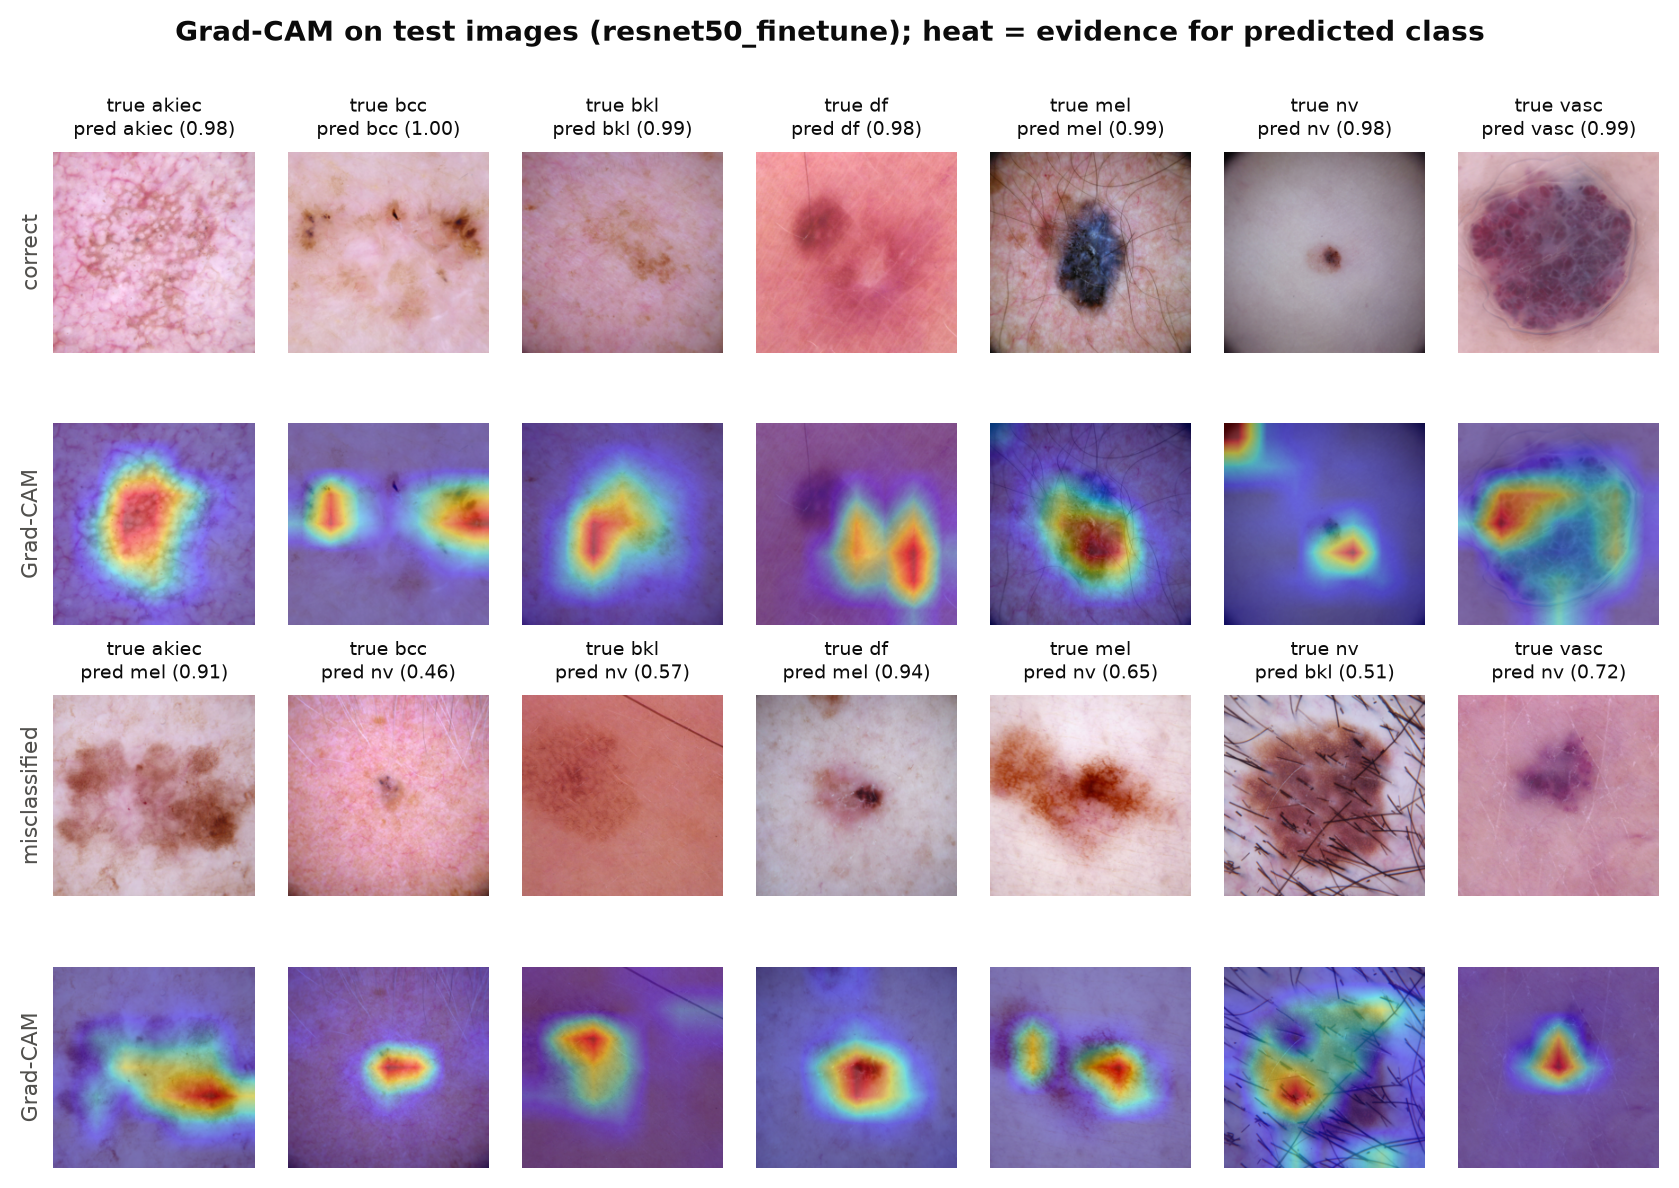
\includegraphics[width=\textwidth]{../results/figures/gradcam_resnet50_finetune.png}
\caption{Grad-CAM~\cite{gradcam} of the final ResNet-50 (last bottleneck block of \texttt{layer4}) on test images.
Rows 1--2: confidently correct examples per class; rows 3--4: one misclassified example per class
(single-view probabilities).}
\label{fig:gradcam}
\end{figure}

\textbf{Grad-CAM} (Figure~\ref{fig:gradcam}) shows that, for most correct predictions, the evidence lies on the
lesion itself:
\begin{itemize}
  \item the scattered pigmented foci of the basal cell carcinoma;
  \item the blue-black centre of the melanoma;
  \item the red-purple lobules of the vascular lesion;
  \item the central lesion area of the actinic keratosis.
\end{itemize}
Two observations call for caution. First, in the correctly classified nevus, a strong activation also sits in the
\emph{dark vignetted corner} of the image, which points to a possible acquisition-artefact shortcut. Second, for
the nevus misclassified as \texttt{bkl}, the heat is spread over the \emph{hairs} covering the lesion. Both point to
hair removal and vignetting-aware cropping as useful preprocessing. Five of the seven misclassified examples are
low-confidence, genuinely ambiguous cases (0.46--0.72). The two exceptions are a pigmented \texttt{akiec}
(0.91) and a \texttt{df} (0.94), both predicted as melanoma.

\begin{figure}[H]
\centering
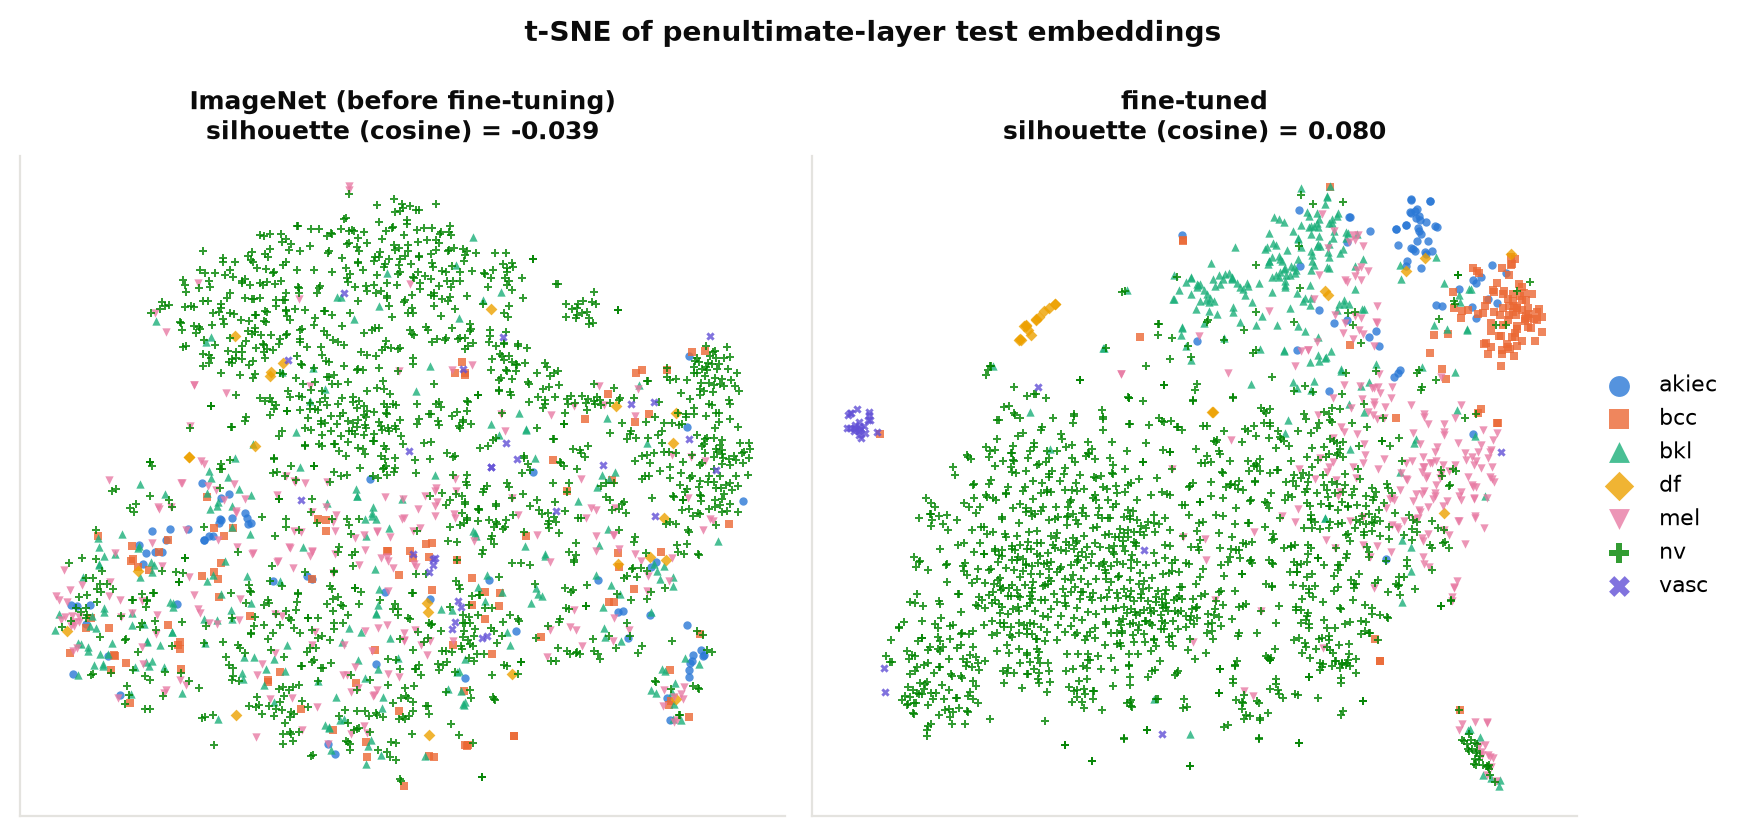
\includegraphics[width=\textwidth]{../results/figures/tsne_resnet50_finetune.png}
\caption{t-SNE~\cite{tsne} of 2048-D penultimate-layer embeddings of the 2{,}005 test images, before (ImageNet
weights) and after fine-tuning. Marker shape and colour both encode the class.}
\label{fig:tsne}
\end{figure}

\textbf{Embeddings.} Figure~\ref{fig:tsne} shows what fine-tuning changes inside the network. With ImageNet
weights, all classes are intermixed (cosine silhouette \SilImageNet). After fine-tuning, \texttt{vasc},
\texttt{df}, \texttt{bcc}, \texttt{akiec} and \texttt{bkl} form compact, separate clusters, and the silhouette
becomes positive (\SilFineTuned). Melanoma occupies a region that borders and overlaps the large nevus cloud,
which matches the \texttt{mel}$\leftrightarrow$\texttt{nv} confusions that dominate the error analysis.

\subsection{Comparison with published DermaMNIST results}
\begin{table}[H]
\centering
\caption{Comparison with the official MedMNIST v2 DermaMNIST benchmark~\cite{medmnistv2}. The MedMNIST v2
baselines were trained on the 28$\times$28 images (the ``224'' variants use 28$\times$28 images upsampled to
224$\times$224); our models use the native 224$\times$224 MedMNIST+ images.}
\label{tab:benchmark}
\small
\begin{tabular}{llrr}
\toprule
Source & Method & Test ACC & Test AUC \\
\midrule
MedMNIST v2 & ResNet-18 (28) / ResNet-18 (224) & 0.735 / 0.754 & 0.917 / 0.920 \\
MedMNIST v2 & ResNet-50 (28) / ResNet-50 (224) & 0.735 / 0.731 & 0.913 / 0.912 \\
MedMNIST v2 & auto-sklearn / AutoKeras & 0.719 / 0.749 & 0.902 / 0.915 \\
MedMNIST v2 & Google AutoML Vision & 0.768 & 0.914 \\
\midrule
This work & SimpleCNN, scratch (E1) & 0.736 & 0.908 \\
This work & EfficientNet-B0, fine-tuned (E5) & 0.848 & 0.959 \\
This work & ResNet-50, fine-tuned (E4) & 0.861 & 0.955 \\
This work & \textbf{ResNet-50, fine-tuned + TTA (final)} & \textbf{0.870} & \textbf{0.962} \\
\bottomrule
\end{tabular}
\end{table}

Our scratch baseline lands in the same range as the MedMNIST v2 baselines (0.72--0.77 ACC), which is a useful
sanity check of the pipeline. The fine-tuned models improve on the best published baseline by about
10 accuracy points and 0.04 AUC. This gain combines two factors, pretraining and native-resolution input, and
the comparison does not separate them. For the effect of pretraining alone, Table~\ref{tab:results} (identical
data and resolution) is the controlled comparison.

\subsection{Computational cost}
All seven runs together took \TotalTrainMin{} minutes of training on the GTX 1660 SUPER (Appendix,
Table~\ref{tab:compute}). A full ResNet-50 fine-tuning epoch takes \RFineEpochTime\,s and peaks at 3.9\,GB of GPU
memory. EfficientNet-B0 needs \EFineEpochTime\,s per epoch, and feature extraction only \EFrozenEpochTime--\RFrozenEpochTime\,s,
because no gradients flow through the backbone.

\section{Discussion and Summary}
\label{sec:summary}

\subsection{Summary of findings}
This assignment studied transfer learning for seven-class dermatoscopic skin-lesion classification on DermaMNIST
(HAM10000, 224$\times$224). Seven controlled experiments led to five conclusions:
\begin{enumerate}
  \item \textbf{Pretraining matters most.} Fine-tuning an ImageNet ResNet-50 lifts test macro-F1 from
        \ScratchFOne\% (CNN trained from scratch) to \RFineFOne\%, and accuracy from \ScratchAcc\% to
        \RFineAcc\%.
  \item \textbf{Fine-tune, do not freeze.} Frozen ImageNet features reach only \RFrozenFOne--\EFrozenFOne\%
        macro-F1. The dermatoscopic domain is far enough from ImageNet that the backbone itself must adapt;
        discriminative learning rates with warm-up make this stable.
  \item \textbf{Gradual unfreezing did not help} in a 12-epoch budget (\RGradFOne\% vs \RFineFOne\%), although it
        is cheaper and ranks well (AUC \RGradAUC).
  \item \textbf{Class weighting trades accuracy and calibration for minority-class recall.} Balanced accuracy goes
        up 4.5 points, \texttt{df}/\texttt{vasc} F1 up 5--6 points, and accuracy down 0.8 points. ECE worsens from
        \RNoWECE{} to \RFineECE.
  \item \textbf{8-view TTA is a reliable, free-to-train gain.} It improves accuracy and AUC for every model.
\end{enumerate}

The final model, \textbf{ResNet-50 with full fine-tuning and 8-view TTA}, selected on validation only, reaches
\textbf{\RFineAccTTA\% accuracy}, \textbf{\RFineBalAccTTA\% balanced accuracy}, \textbf{\RFineFOneTTA\% macro-F1}
(95\% CI \RFineFOneTTACI) and \textbf{macro-AUC \RFineAUCTTA} on the held-out test set. That is about 10 accuracy
points above the best result in the official MedMNIST v2 benchmark table. It detects \BestRecMel\% of melanomas,
and its errors are concentrated in the clinically hard \texttt{mel}/\texttt{nv} and
\texttt{akiec}/\texttt{bkl} pairs. Grad-CAM shows that its evidence usually lies on the lesion itself.

\subsection{Limitations}
\label{sec:limitations}
\begin{itemize}
  \item \textbf{Same-lesion leakage.} The official split is image-level. Our audit (Section~\ref{sec:leakage})
        found re-photographed training lesions in the test set, so the absolute scores are probably slightly
        optimistic. A lesion-level split needs the HAM10000 metadata, which DermaMNIST does not ship.
  \item \textbf{Single seed and single split.} Each configuration was trained once (seed 42). The bootstrap CIs
        capture test-set sampling noise but not training variance. Several of the closer comparisons
        (ResNet-50 vs EfficientNet-B0, weighted vs unweighted) overlap within their CIs and should be repeated
        over 3--5 seeds before drawing firm conclusions.
  \item \textbf{Limited tuning budget.} Learning rates, epochs and the unfreezing schedule were set from common
        practice, not searched, because of the 6\,GB GPU. Gradual unfreezing in particular might do better with a
        longer schedule.
  \item \textbf{Under-confident probabilities.} The final model's raw probabilities are under-confident (ECE
        \RFineECETTA) and should be temperature-scaled before being read as risk scores.
  \item \textbf{Dataset scope.} HAM10000 comes from two centres and mostly fair skin types. Performance on darker
        skin, on other dermatoscopes, or on clinical (non-dermatoscopic) photographs is untested.
\end{itemize}

\subsection{Ethical considerations}
This is a course project on a public research dataset (CC BY-NC 4.0). It is \emph{not} a medical device and must
not be used for diagnosis. In any clinical use, the most costly error is a missed melanoma, so recall on the
malignant classes and calibrated uncertainty matter more than overall accuracy. The model would also need
validation across skin types to avoid unequal performance between patient groups.

\subsection{Future work}
\begin{itemize}
  \item Re-split by lesion using HAM10000 metadata and re-evaluate, to remove the leakage.
  \item Repeat every run over 5 seeds and report mean $\pm$ standard deviation; tune per-class decision thresholds
        and the temperature on the validation split.
  \item Add hair-removal and vignette-aware preprocessing, which Grad-CAM suggests is needed.
  \item Compare stronger backbones (ConvNeXt, Vision Transformers, dermatology-specific foundation models) and
        larger input sizes using the same pipeline~\cite{medmnistplus}.
  \item Test external generalisation on ISIC 2019/2020 images.
\end{itemize}

\subsection{Conclusion}
For a small, imbalanced medical-imaging dataset, ImageNet transfer learning with \emph{full} fine-tuning and
discriminative learning rates turned a weak from-scratch baseline (\ScratchFOne\% macro-F1) into a strong
classifier (\RFineFOneTTA\% macro-F1, \RFineAccTTA\% accuracy with TTA). This was done on a single 6\,GB consumer
GPU in about an hour of total training. The comparison also shows that the details matter: whether to freeze
or fine-tune, how to handle class imbalance, and how to evaluate (macro-F1, confidence intervals, calibration,
leakage checks). These choices change both the numbers and the conclusions one should draw from them.

\section{Codebase}
\label{sec:codebase}

\textbf{Repository:} \href{\repo}{\texttt{\repo}}

The repository contains all source code, the experiment script, the per-epoch training logs, evaluation
outputs (JSON), every figure, and the \LaTeX{} source of this report. Model checkpoints and the dataset are
excluded because of their size; \texttt{scripts/run\_all.sh} downloads the data and regenerates both.

\subsection*{Repository layout}
\begin{lstlisting}
dermamnist-transfer-learning/
|-- src/
|   |-- common.py          paths, class names, memory-mapped Dataset, augmentation, class weights
|   |-- prepare_data.py    MD5-checked .npz -> per-split .npy conversion
|   |-- eda.py             data analysis + figures + duplicate/leakage audit
|   |-- models.py          SimpleCNN, ResNet-50, EfficientNet-B0, stage split, embeddings
|   |-- train.py           scratch / frozen / finetune / gradual training with model selection
|   |-- metrics.py         accuracy, balanced acc., macro-F1, AUC, ECE, bootstrap CIs
|   |-- evaluate.py        test evaluation with and without 8-view TTA
|   |-- make_figures.py    comparison figures and LaTeX tables
|   |-- gradcam.py         Grad-CAM and t-SNE for the selected model
|   |-- report_numbers.py  numbers quoted in this report, as LaTeX macros
|   `-- plot_style.py      shared colour-blind-safe figure style
|-- scripts/run_all.sh     reproduces every experiment, table and figure
|-- results/               eda.json, summary.json, runs/<name>/{config,history,eval}, figures/, logs/
|-- report/                LaTeX source and compiled PDF of this report
`-- requirements.txt
\end{lstlisting}

\subsection*{Reproducing the results}
\begin{lstlisting}
git clone https://github.com/mr-shakib/dermamnist-transfer-learning.git
cd dermamnist-transfer-learning
python3.12 -m venv .venv
.venv/bin/pip install torch torchvision --index-url https://download.pytorch.org/whl/cu126
.venv/bin/pip install -r requirements.txt
bash scripts/run_all.sh          # about 70 min on a GTX 1660 SUPER
cd report && latexmk -pdf main.tex
\end{lstlisting}

\begin{thebibliography}{99}
\addcontentsline{toc}{section}{References}
\small

\bibitem{ham10000} P.~Tschandl, C.~Rosendahl, and H.~Kittler, ``The HAM10000 dataset, a large collection of
multi-source dermatoscopic images of common pigmented skin lesions,'' \emph{Scientific Data}, vol.~5, art.~180161,
2018.

\bibitem{isic2018} N.~Codella \emph{et al.}, ``Skin lesion analysis toward melanoma detection 2018: A challenge
hosted by the International Skin Imaging Collaboration (ISIC),'' arXiv:1902.03368, 2019.

\bibitem{medmnistv2} J.~Yang, R.~Shi, D.~Wei, Z.~Liu, L.~Zhao, B.~Ke, H.~Pfister, and B.~Ni, ``MedMNIST v2 -- A
large-scale lightweight benchmark for 2D and 3D biomedical image classification,'' \emph{Scientific Data},
vol.~10, art.~41, 2023.

\bibitem{medmnistplus} S.~Doerrich, F.~Di~Salvo, J.~Brockmann, and C.~Ledig, ``Rethinking model prototyping
through the MedMNIST+ dataset collection,'' \emph{Scientific Reports}, vol.~15, art.~7669, 2025,
doi:10.1038/s41598-025-92156-9.

\bibitem{esteva2017} A.~Esteva, B.~Kuprel, R.~A.~Novoa, J.~Ko, S.~M.~Swetter, H.~M.~Blau, and S.~Thrun,
``Dermatologist-level classification of skin cancer with deep neural networks,'' \emph{Nature}, vol.~542,
pp.~115--118, 2017.

\bibitem{imagenet} J.~Deng, W.~Dong, R.~Socher, L.-J.~Li, K.~Li, and L.~Fei-Fei, ``ImageNet: A large-scale
hierarchical image database,'' in \emph{Proc.\ CVPR}, 2009.

\bibitem{vgg} K.~Simonyan and A.~Zisserman, ``Very deep convolutional networks for large-scale image
recognition,'' in \emph{Proc.\ ICLR}, 2015.

\bibitem{resnet} K.~He, X.~Zhang, S.~Ren, and J.~Sun, ``Deep residual learning for image recognition,'' in
\emph{Proc.\ CVPR}, pp.~770--778, 2016.

\bibitem{efficientnet} M.~Tan and Q.~V.~Le, ``EfficientNet: Rethinking model scaling for convolutional neural
networks,'' in \emph{Proc.\ ICML}, pp.~6105--6114, 2019.

\bibitem{yosinski2014} J.~Yosinski, J.~Clune, Y.~Bengio, and H.~Lipson, ``How transferable are features in deep
neural networks?'' in \emph{Advances in NeurIPS}, 2014.

\bibitem{kornblith2019} S.~Kornblith, J.~Shlens, and Q.~V.~Le, ``Do better ImageNet models transfer better?''
in \emph{Proc.\ CVPR}, 2019.

\bibitem{raghu2019} M.~Raghu, C.~Zhang, J.~Kleinberg, and S.~Bengio, ``Transfusion: Understanding transfer
learning for medical imaging,'' in \emph{Advances in NeurIPS}, 2019.

\bibitem{ulmfit} J.~Howard and S.~Ruder, ``Universal language model fine-tuning for text classification,'' in
\emph{Proc.\ ACL}, 2018.

\bibitem{labelsmoothing} C.~Szegedy, V.~Vanhoucke, S.~Ioffe, J.~Shlens, and Z.~Wojna, ``Rethinking the Inception
architecture for computer vision,'' in \emph{Proc.\ CVPR}, 2016.

\bibitem{adamw} I.~Loshchilov and F.~Hutter, ``Decoupled weight decay regularization,'' in \emph{Proc.\ ICLR},
2019.

\bibitem{sgdr} I.~Loshchilov and F.~Hutter, ``SGDR: Stochastic gradient descent with warm restarts,'' in
\emph{Proc.\ ICLR}, 2017.

\bibitem{guo2017} C.~Guo, G.~Pleiss, Y.~Sun, and K.~Q.~Weinberger, ``On calibration of modern neural networks,''
in \emph{Proc.\ ICML}, 2017.

\bibitem{gradcam} R.~R.~Selvaraju, M.~Cogswell, A.~Das, R.~Vedantam, D.~Parikh, and D.~Batra, ``Grad-CAM: Visual
explanations from deep networks via gradient-based localization,'' in \emph{Proc.\ ICCV}, 2017.

\bibitem{tsne} L.~van~der~Maaten and G.~Hinton, ``Visualizing data using t-SNE,'' \emph{Journal of Machine
Learning Research}, vol.~9, pp.~2579--2605, 2008.

\bibitem{pytorch} A.~Paszke \emph{et al.}, ``PyTorch: An imperative style, high-performance deep learning
library,'' in \emph{Advances in NeurIPS}, 2019.

\end{thebibliography}

\appendix
\section{Additional results}
\label{app:extra}

\subsection{Effect of test-time augmentation on every run}
\begin{table}[H]
\centering
\caption{Test metrics without and with 8-view dihedral TTA (4 rotations $\times$ horizontal flip, softmax
averaged).}
\label{tab:tta}
\small
\begin{tabular}{lrrrrrr}
\toprule
 & \multicolumn{2}{c}{Accuracy (\%)} & \multicolumn{2}{c}{Macro-F1 (\%)} & \multicolumn{2}{c}{Macro-AUC} \\
\cmidrule(lr){2-3}\cmidrule(lr){4-5}\cmidrule(lr){6-7}
Run & single & TTA & single & TTA & single & TTA \\
\midrule
\inputrows{generated/tta_table.tex}
\bottomrule
\end{tabular}
\end{table}

\subsection{Training cost}
\begin{table}[H]
\centering
\caption{Training cost on the GTX 1660 SUPER (FP32, batch 32). Peak memory is the PyTorch allocator peak,
including the cuDNN workspace.}
\label{tab:compute}
\small
\begin{tabular}{lrrr}
\toprule
Run & s / epoch & train time (min) & peak GPU mem.\ (GB) \\
\midrule
\inputrows{generated/compute_table.tex}
\bottomrule
\end{tabular}
\end{table}

\subsection{Common hyper-parameters}
\begin{table}[H]
\centering
\caption{Hyper-parameters shared by all runs.}
\label{tab:hparams}
\begin{tabularx}{\textwidth}{lX}
\toprule
Input & $224\times224$ RGB, ImageNet mean/std normalisation \\
Train augmentation & RandomResizedCrop (scale 0.75--1, ratio 0.9--1.1), H/V flip, rot90, ColorJitter (0.2, 0.2, 0.15, 0.02) \\
Optimiser & AdamW, $\beta=(0.9,0.999)$, weight decay $10^{-4}$, gradient clip 5.0 \\
Schedule & 1-epoch linear warm-up, cosine decay to 0 (per step) \\
Batch size & 32 (train), 64 (evaluation) \\
Loss & cross-entropy, label smoothing 0.05, $\sqrt{\text{inverse-frequency}}$ class weights \\
Regularisation & dropout 0.3 before the classifier, weight decay, augmentation \\
Selection & best validation macro-F1; early-stopping patience 6 (8 for scratch) \\
Seed & 42 \\
\bottomrule
\end{tabularx}
\end{table}


\end{document}
